\documentclass[a4paper,12pt]{article}
%\documentclass[fleqn]{article}

% ---パッケージ---
\usepackage{amsmath,amssymb}    %数式用
\usepackage{tcolorbox}   %囲み枠用(tcolorboxに変更)
\usepackage{geometry}   %余白調節
\usepackage{tikz}  % ← 図を描くためのTikZパッケージ
\geometry{margin=25mm}  %余白を少し狭く
\usetikzlibrary{decorations.pathmorphing,patterns,positioning,arrows.meta} % バネ・壁の模様
\tikzset{
  block/.style = {draw, rectangle, minimum height=2em, minimum width=3em},
  sum/.style = {draw, circle, inner sep=0pt, minimum size=5mm},
  input/.style = {coordinate},
  output/.style = {coordinate}
}
\usetikzlibrary{calc}

% --- 日本語用パッケージ ---
\usepackage{luatexja}         % 日本語表示に必要
\usepackage{luatexja-fontspec} % フォント指定用

% --- フォント指定(Overleaf標準フォント)---
\setmainjfont{IPAexMincho}  % 明朝体
%\setmainjfont{IPAexGothic}  % ゴシック体にしたい場合

% --- tcolorbox の設定 ---
\tcbset{
  colframe=black,
  colback=white,         % 本文の背景(白)
  boxrule=0.8pt,
  arc=3pt,
  outer arc=3pt,
  boxsep=4pt,
  coltitle=black,
  colbacktitle=gray!20,  % タイトルの背景(グレー)
  fonttitle=\normalsize
}

\begin{document}

% --------------- [41] --------------- 済
\begin{tcolorbox}[title={[41] 出力信号である制御量\(Y\)までの伝達特性を等価変換によって簡単化せよ.\\
  \qquad ただし、\(R\)は目標値信号,\(D\)は外乱信号である.
\begin{center}
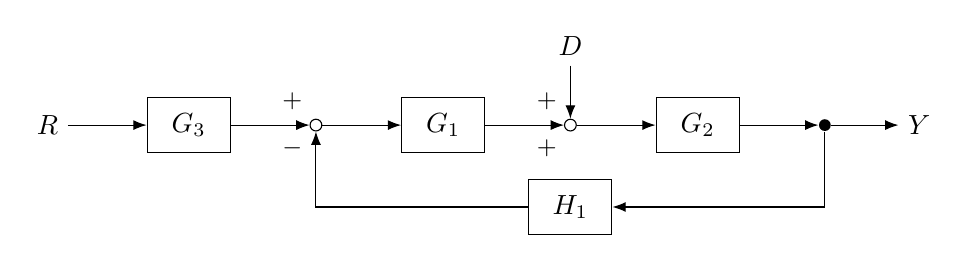
\begin{tikzpicture}[auto, node distance=0.8cm and 1.0cm, >=Latex]

  % --- ノードと信号配置(横並び) ---
  \node at (0,0) (R) {$R$};                           % R(目標値)
  \node[block, right=of R] (G3) {$G_3$};              % G3
  \node[circle, draw, inner sep=1.5pt, right=of G3] (sum1) {};  % 合流点1
  \node[block, right=of sum1] (G1) {$G_1$};           % G1
  \node[circle, draw, inner sep=1.5pt, right=of G1] (sum2) {};  % 合流点2
  \node[block, right=of sum2] (G2) {$G_2$};           % G2
  \node[circle, fill=black, inner sep=1.5pt, right=of G2] (branch) {}; % 分岐点
  \node at ($(branch)+(1.2,0)$) (Y) {$Y$};             % Y(制御量)

  % --- 上下ノード ---
  \node at ($(sum2)+(0,1.0)$) (D) {$D$};               % D(外乱)
  \node[block, below=0.6cm of sum2] (H1) {$H_1$};      % H1(下)

  % === 経路 ===
  \draw[->] (R) -- (G3);
  \draw[->] (G3) -- (sum1);
  \draw[->] (sum1) -- (G1);
  \draw[->] (G1) -- (sum2);
  \draw[->] (sum2) -- (G2);
  \draw[->] (G2) -- (branch);
  \draw[->] (branch) -- (Y);

  \draw[->] (D) -- (sum2);            % D → 合流点2
  \draw[->] (branch) |- (H1);         % 分岐 → H1(下)
  \draw[->] (H1) -| (sum1);           % H1 → 合流点1(戻る)

  % --- 加算記号配置 ---
  \node at ($(sum1)+(-0.3,0.3)$) {\small $+$};
  \node at ($(sum1)+(-0.3,-0.3)$) {\small $-$};
  \node at ($(sum2)+(-0.3,0.3)$) {\small $+$};
  \node at ($(sum2)+(-0.3,-0.3)$) {\small $+$};

\end{tikzpicture}
\end{center}
}]
%------- RからY -------
RからYについて
\begin{center}

  % --- Step 1:G₁とG₂のみを合成、G₃とH₁はそのまま配置 ---
  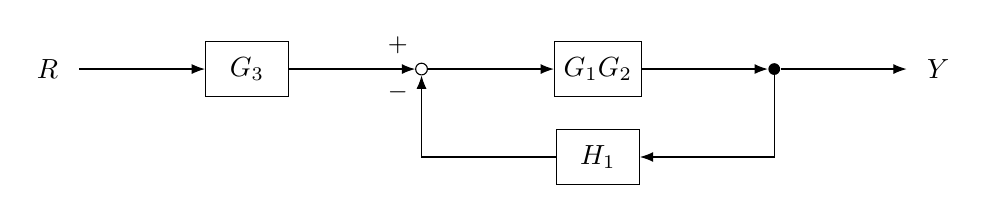
\begin{tikzpicture}[auto, node distance=1.2cm and 1.6cm, >=Latex]
  
    \node[input] (R) {};
    \node[block, right=of R] (G3) {$G_3$};
    \node[circle, draw, inner sep=1.5pt, right=of G3] (sum1) {};
    \node[block, right=of sum1] (G1G2) {$G_1 G_2$};
    \node[circle, fill=black, inner sep=1.5pt, right=of G1G2] (branch) {};
    \node[output, right=of branch] (Y) {};
  
    \node[block, below=0.4cm of G1G2] (H1) {$H_1$};
  
    \draw[->] (R) -- (G3);
    \draw[->] (G3) -- (sum1);
    \draw[->] (sum1) -- (G1G2);
    \draw[->] (G1G2) -- (branch);
    \draw[->] (branch) -- (Y);
  
    \draw[->] (branch) |- (H1);
    \draw[->] (H1) -| (sum1);
  
    \node at ($(sum1)+(-0.3,0.3)$) {\small $+$};
    \node at ($(sum1)+(-0.3,-0.3)$) {\small $-$};
    \node at ($(R)+(-0.4,0)$) {$R$};
    \node at ($(Y)+(0.4,0)$) {$Y$};

  
  \end{tikzpicture}

  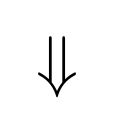
\begin{tikzpicture}
    \node {\Huge$\Downarrow$};
  \end{tikzpicture}

  
  % --- Step 2:H₁との負帰還構造を合成(G₃はまだ分離) ---
  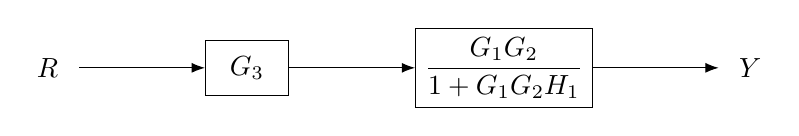
\begin{tikzpicture}[auto, node distance=1.2cm and 1.6cm, >=Latex]
  
    \node[input] (R) {};
    \node[block, right=of R] (G3) {$G_3$};
    \node[block, right=of G3] (closedLoop) {$\dfrac{G_1 G_2}{1 + G_1 G_2 H_1}$};
    \node[output, right=of closedLoop] (Y) {};
  
    \draw[->] (R) -- (G3);
    \draw[->] (G3) -- (closedLoop);
    \draw[->] (closedLoop) -- (Y);

    \node at ($(R)+(-0.4,0)$) {$R$};
    \node at ($(Y)+(0.4,0)$) {$Y$};

  
  \end{tikzpicture}
  

  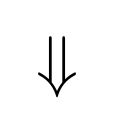
\begin{tikzpicture}
    \node {\Huge$\Downarrow$};
  \end{tikzpicture}

  
  % --- Step 3:G₃を含めた全体の1ブロック化 ---
  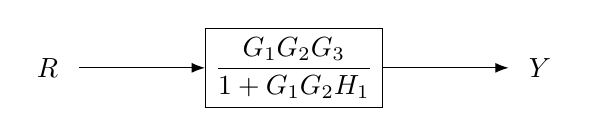
\begin{tikzpicture}[auto, node distance=1.4cm and 1.6cm, >=Latex]
  
    \node[input] (R) {};
    \node[block, right=of R] (total) {$\dfrac{G_1 G_2 G_3}{1 + G_1 G_2 H_1}$};
    \node[output, right=of total] (Y) {};
  
    \draw[->] (R) -- (total);
    \draw[->] (total) -- (Y);

    \node at ($(R)+(-0.4,0)$) {$R$};
    \node at ($(Y)+(0.4,0)$) {$Y$};
  
  \end{tikzpicture}
  
  \end{center}

%------- DからY -------
DからYについて
\begin{center}

  % --- Step 0:G₂ → G₁ → 分岐 → H₁ → 合流点(D入力) ---
  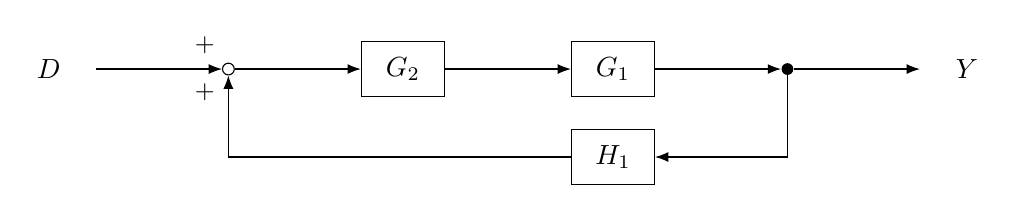
\begin{tikzpicture}[auto, node distance=1.2cm and 1.6cm, >=Latex]
  
    \node[input] (D) {};
    \node[circle, draw, inner sep=1.5pt, right=of D] (sum2) {};
    \node[block, right=of sum2] (G2) {$G_2$};
    \node[block, right=of G2] (G1) {$G_1$};
    \node[circle, fill=black, inner sep=1.5pt, right=of G1] (branch) {};
    \node[output, right=of branch] (Y) {};
    \node[block, below=0.4cm of G1] (H1) {$H_1$};
  
    \draw[->] (D) -- (sum2);
    \draw[->] (sum2) -- (G2);
    \draw[->] (G2) -- (G1);
    \draw[->] (G1) -- (branch);
    \draw[->] (branch) -- (Y);
  
    \draw[->] (branch) |- (H1);
    \draw[->] (H1) -| (sum2);
  
    \node at ($(D)+(-0.6,0)$) {$D$};
    \node at ($(Y)+(0.6,0)$) {$Y$};
    \node at ($(sum2)+(-0.3,0.3)$) {\small $+$};
    \node at ($(sum2)+(-0.3,-0.3)$) {\small $+$};
  
  \end{tikzpicture}

  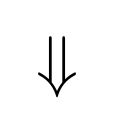
\begin{tikzpicture}
    \node {\Huge$\Downarrow$};
  \end{tikzpicture}
  
  % --- Step 1:G₁とG₂を合成(H₁と構造はそのまま) ---
  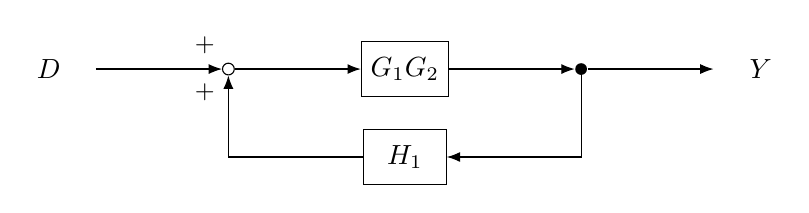
\begin{tikzpicture}[auto, node distance=1.2cm and 1.6cm, >=Latex]
  
    \node[input] (D) {};
    \node[circle, draw, inner sep=1.5pt, right=of D] (sum2) {};
    \node[block, right=of sum2] (G1G2) {$G_1 G_2$};
    \node[circle, fill=black, inner sep=1.5pt, right=of G1G2] (branch) {};
    \node[output, right=of branch] (Y) {};
    \node[block, below=0.4cm of G1G2] (H1) {$H_1$};
  
    \draw[->] (D) -- (sum2);
    \draw[->] (sum2) -- (G1G2);
    \draw[->] (G1G2) -- (branch);
    \draw[->] (branch) -- (Y);
  
    \draw[->] (branch) |- (H1);
    \draw[->] (H1) -| (sum2);
  
    \node at ($(D)+(-0.6,0)$) {$D$};
    \node at ($(Y)+(0.6,0)$) {$Y$};
    \node at ($(sum2)+(-0.3,0.3)$) {\small $+$};
    \node at ($(sum2)+(-0.3,-0.3)$) {\small $+$};
  
  \end{tikzpicture}
  
  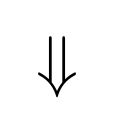
\begin{tikzpicture}
    \node {\Huge$\Downarrow$};
  \end{tikzpicture}
  
  % --- Step 2:全体を1ブロックに簡約(D→Y) ---
  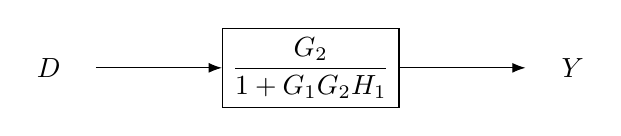
\begin{tikzpicture}[auto, node distance=1.4cm and 1.6cm, >=Latex]
  
    \node[input] (D) {};
    \node[block, right=of D] (total) {$\dfrac{G_2}{1 + G_1 G_2 H_1}$};
    \node[output, right=of total] (Y) {};
  
    \draw[->] (D) -- (total);
    \draw[->] (total) -- (Y);
  
    \node at ($(D)+(-0.6,0)$) {$D$};
    \node at ($(Y)+(0.6,0)$) {$Y$};
  
  \end{tikzpicture}
  
  \end{center}

  これらを合わせて
  \[
  Y=\frac{G_1 G_2 G_3 R + G_2 D}{1+G_1 G_2 H_1}\]
  
  
\end{tcolorbox}
% --------------- [42] --------------- 済
\begin{tcolorbox}[title={[42] \(a\)を入力,\(b\)を出力としたとき,ブロック線図を簡単化し,伝達関数を求めよ. 
  \begin{center}
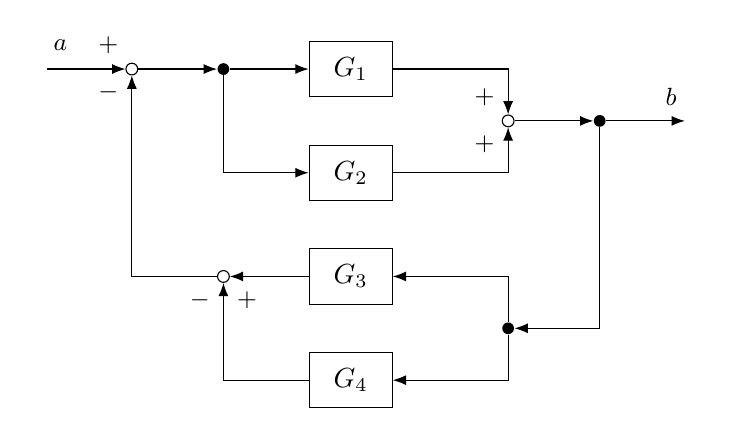
\begin{tikzpicture}[auto, node distance=0.8cm and 1.0cm, >=Latex]

  % --- 上段:主系列ノード ---
  \node at (0,0) (input) {};
  \node[circle, draw, inner sep=1.5pt, right=of input] (sum1) {};               % 合流1
  \node[circle, fill=black, inner sep=1.5pt, right=of sum1] (branch1) {};       % 分岐1
  \node[block, right=of branch1] (G1) {$G_1$};                                   % G1

  % --- 縦系列:G2〜G4 ---
  \node[block, below=0.6cm of G1] (G2) {$G_2$};
  \node[block, below=0.6cm of G2] (G3) {$G_3$};
  \node[block, below=0.6cm of G3] (G4) {$G_4$};

  % --- G1とG2の中間に sum2 → branch2 → output ---
  \coordinate (mid12) at ($(G1)!0.5!(G2)$);
  \node[circle, draw, inner sep=1.5pt] at ($(mid12)+(2.0,0)$) (sum2) {};        % 合流2
  \node[circle, fill=black, inner sep=1.5pt, right=of sum2] (branch2) {};       % 分岐2
  \node[right=of branch2] (output) {};

  % --- G3とG4の中間に branch3 ---
  \coordinate (mid34) at ($(G3)!0.5!(G4)$);
  \node[circle, fill=black, inner sep=1.5pt] at ($(mid34)+(2.0,0)$) (branch3) {}; % 分岐3

% --- branch1の下かつG3の左に合流3 ---
\node[circle, draw, inner sep=1.5pt, left=of G3] (sum3) {};% 合流3
  
  % === 経路 ===
  \draw[->] (input) -- (sum1);
  \draw[->] (sum1) -- (branch1);
  \draw[->] (branch1) -- (G1);
  \draw[->] (G1) -| (sum2);
  \draw[->] (sum2) -- (branch2);
  \draw[->] (branch2) -- (output);

  \draw[->] (branch1) |- (G2);
  \draw[->] (G2) -| (sum2);

  \draw[->] (branch2) |- (branch3);
  \draw[->] (branch3) |- (G3);
  \draw[->] (G3) -- (sum3);
  \draw[->] (sum3) -| (sum1);

  \draw[->] (branch3) |- (G4);
  \draw[->] (G4) -| (sum3);

  % --- 加算記号 ---
  \node at ($(sum1)+(-0.3,0.3)$) {\small $+$};
  \node at ($(sum1)+(-0.3,-0.3)$) {\small $-$};
  \node at ($(sum2)+(-0.3,0.3)$) {\small $+$};
  \node at ($(sum2)+(-0.3,-0.3)$) {\small $+$};
  \node at ($(sum3)+(-0.3,-0.3)$) {\small $-$};
  \node at ($(sum3)+(0.3,-0.3)$) {\small $+$};

  % --- その他記号 ---
  \node at ($(input)+(0.3,0.3)$) {\small $a$};
  \node at ($(output)+(-0.3,0.3)$) {\small $b$};

\end{tikzpicture}
  \end{center}
  }]

  \begin{center}

    % --- Step 1:G₁+G₂,G₄−G₃ に合成した構造 ---
    \begin{tikzpicture}[auto, node distance=1.2cm and 1.8cm, >=Latex]

      \node[input] (input) {};
      \node[circle, draw, inner sep=1.5pt, right=of input] (sum1) {};
      \node[block, right=of sum1] (G1G2) {$G_1 + G_2$};
      \node[circle, fill=black, inner sep=1.5pt, right=of G1G2] (branch) {};
      \node[output, right=of branch] (output) {};
      \node[block, below=1.2cm of G1G2] (G3minusG4) {$G_3 - G_4$};
    
      \draw[->] (input) -- (sum1);
      \draw[->] (sum1) -- (G1G2);
      \draw[->] (G1G2) -- (branch);
      \draw[->] (branch) -- (output);
    
      \draw[->] (branch) |- (G3minusG4);
      \draw[->] (G3minusG4) -| (sum1);
    
      % ラベル配置
      \node at ($(input)+(0.3,0.3)$) {\small $a$};
      \node at ($(output)+(-0.3,0.3)$) {\small $b$};
    
      % 加算記号
      \node at ($(sum1)+(-0.3,0.3)$) {\small $+$};
      \node at ($(sum1)+(-0.3,-0.3)$) {\small $-$};
    
    \end{tikzpicture}
    
    \vspace{0.2cm}
    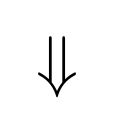
\begin{tikzpicture}
      \node {\Huge$\Downarrow$};
    \end{tikzpicture}
    \vspace{0.2cm}
    
    % --- Step 2:全体を1ブロックに簡約 ---
    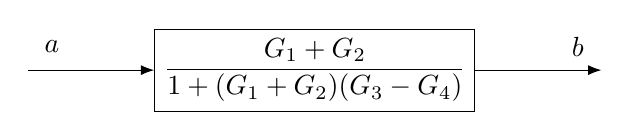
\begin{tikzpicture}[auto, node distance=1.6cm and 1.6cm, >=Latex]
    
      \node[input] (a) {};
      \node[block, right=of a] (TF) {$\dfrac{G_1 + G_2}{1 + (G_1 + G_2)(G_3 - G_4)}$};
      \node[output, right=of TF] (b) {};
    
      \draw[->] (a) -- (TF);
      \draw[->] (TF) -- (b);
    
      \node at ($(a)+(0.3,0.3)$) {$a$};
      \node at ($(b)+(-0.3,0.3)$) {$b$};
    
    \end{tikzpicture}
    
    \end{center}
    

\end{tcolorbox}
% --------------- [43] --------------- 済
\begin{tcolorbox}[title={[43] 伝達関数\(\frac{b(s)}{a(s)}\)を求めよ. 
  \begin{center}
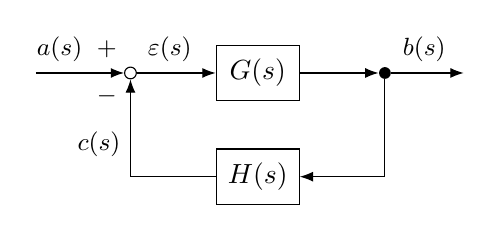
\begin{tikzpicture}[auto, node distance=0.8cm and 1.0cm, >=Latex]

  % --- 横並びノード ---
  \node[circle, draw, inner sep=1.5pt] (sum) {};                  % 合流点
  \node[block, right=of sum] (G) {$G(s)$};                        % G(s)
  \node[circle, fill=black, inner sep=1.5pt, right=of G] (branch) {};  % 分岐点

  % --- 下段ノード ---
  \node[block, below=0.6cm of G] (H) {$H(s)$};                    % H(s)

  % --- 経路 ---
  \draw[->] ++(-1.2,0) -- (sum);              % input → 合流点
  \draw[->] (sum) -- (G);                     % 合流点 → G(s)
  \draw[->] (G) -- (branch);                  % G(s) → 分岐点
  \draw[->] (branch) -- ++(1.0,0);            % 分岐点 → output

  \draw[->] (branch) |- (H);                  % 分岐点 → H(s)
  \draw[->] (H) -| (sum);                     % H(s) → 合流点

  % --- 加算記号 ---
  \node at ($(sum)+(-0.3,0.3)$) {\small $+$};
  \node at ($(sum)+(-0.3,-0.3)$) {\small $-$};

  % --- その他記号 ---
  \node at ($(sum)+(-0.9,0.3)$) {\small $a(s)$};
  \node at ($(sum)+(0.5,0.3)$) {\small $\varepsilon(s)$};
  \node at ($(branch)+(0.5,0.3)$) {\small $b(s)$};
  \node at ($(sum)+(-0.4,-0.9)$) {\small $c(s)$};
\end{tikzpicture}
  \end{center}
  }]

  ブロック線図より次が成り立つ
  \[
  \left\{
  \begin{aligned}
    \varepsilon(s) &=a(s) - c(s) \qquad \cdot \cdot \cdot (1)\\
    b(s) &=\varepsilon(s) G(s) \qquad \quad \cdot \cdot \cdot (2)\\
    c(s) &=b(s)H(s)\qquad \quad \cdot \cdot \cdot (3)\\
  \end{aligned}
  \right.
  \]
  であるから、最終的に\(\varepsilon(s),c(s)\)を含まない形にするために
  \(\varepsilon(s)\)について解くと\\
  \((1),(3)\)より
  \begin{align*}
  \varepsilon(s) &=a(s) - b(s)H(s)\qquad \quad \cdot \cdot \cdot (4)
  \end{align*}
  よって\((2),(4)\)より
  \begin{align*}
    &\qquad \frac{b(s)}{G(s)} =\varepsilon(s) \\
    &\Leftrightarrow \frac{b(s)}{G(s)} =a(s) - b(s)H(s) \\
    &\Leftrightarrow b(s) = a(s)G(s)-b(s)H(s)G(s) \\
    &\Leftrightarrow b(s)\left\{1+G(s)H(s)\right\} = a(s)G(s) \\
    &\Leftrightarrow \frac{b(s)}{a(s)} = \frac{G(s)}{1+G(s)H(s)}
  \end{align*}


\end{tcolorbox}
% --------------- [44] --------------- 済
\begin{tcolorbox}[title={[44] 二つの入力信号\(a_1(s),a_2(s)\)をもつ,制御系の応答\(b(s)\)を求めよ.
  \begin{center}
  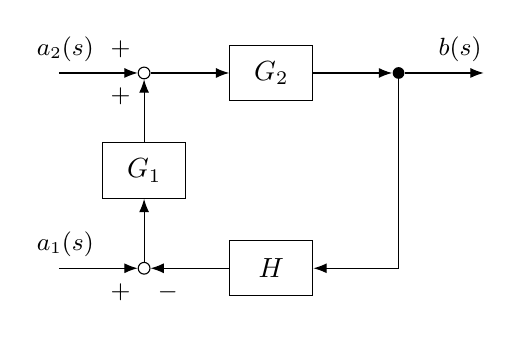
\begin{tikzpicture}[auto, node distance=0.8cm and 1.0cm, >=Latex]

    % --- 上段ノード(横並び) ---
    \node[circle, draw, inner sep=1.5pt] (sum1) {};                % 合流点1
    \node[block, right=of sum1] (G1) {$G_2$};                      % G1
    \node[circle, fill=black, inner sep=1.5pt, right=of G1] (branch) {}; % 分岐点

    % input1とoutputの位置(描かない)
    \coordinate[left=of sum1] (input1);
    \coordinate[right=of branch] (output);

    % --- 中央の縦ノード(合流1 → G2 → 合流2) ---
    \node[block, below=0.8cm of sum1] (G2) {$G_1$};                % G2
    \node[circle, draw, inner sep=1.5pt, below=0.8cm of G2] (sum2) {}; % 合流点2

    % --- 下段(横並び) ---
    \coordinate[left=of sum2] (input2);                            % input2(描かない)
    \node[block, right=of sum2] (H) {$H$};                         % H

    % === 経路 ===
    \draw[->] (input1) -- (sum1);          % input1 → 合流点1
    \draw[->] (sum1) -- (G1);              % 合流点1 → G1
    \draw[->] (G1) -- (branch);            % G1 → 分岐点
    \draw[->] (branch) -- (output);        % 分岐点 → 出力

    \draw[->] (branch) |- (H);             % 分岐点 → H
    \draw[->] (H) -- (sum2);               % H → 合流点2
    \draw[->] (sum2) -- (G2);              % 合流点2 → G2
    \draw[->] (G2) -- (sum1);              % G2 → 合流点1

    \draw[->] (input2) -- (sum2);          % input2 → 合流点2

    % --- 加算記号配置 ---
    \node at ($(sum1)+(-0.3,0.3)$) {\small $+$};
    \node at ($(sum1)+(-0.3,-0.3)$) {\small $+$};
    \node at ($(sum2)+(-0.3,-0.3)$) {\small $+$};
    \node at ($(sum2)+(0.3,-0.3)$) {\small $-$};

    % --- その他記号配置 ---
    \node at ($(sum1)+(-1.0,0.3)$) {\small $a_2(s)$};
    \node at ($(sum2)+(-1.0,0.3)$) {\small $a_1(s)$};
    \node at ($(output)+(-0.3,0.3)$) {\small $b(s)$};

  \end{tikzpicture}
  \end{center}
  }]

  \(a_2(s)=0\)とおくと

  \begin{center}
    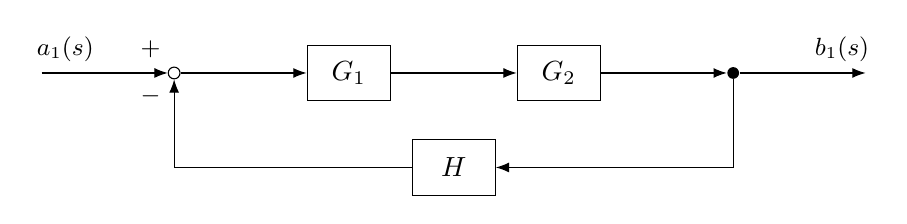
\begin{tikzpicture}[auto, node distance=1.2cm and 1.6cm, >=Latex]
    
      \node[input] (a1) {};
      \node[circle, draw, inner sep=1.5pt, right=of a1] (sum) {};
      \node[block, right=of sum] (G1) {$G_1$};
      \node[block, right=of G1] (G2) {$G_2$};
      \node[circle, fill=black, inner sep=1.5pt, right=of G2] (branch) {};
      \node[output, right=of branch] (b1) {};
    
      \node[block] at ($(G1)!0.5!(G2)+(0,-1.2)$) (H) {$H$};
    
      \draw[->] (a1) -- (sum);
      \draw[->] (sum) -- (G1);
      \draw[->] (G1) -- (G2);
      \draw[->] (G2) -- (branch);
      \draw[->] (branch) -- (b1);
    
      \draw[->] (branch) |- (H);
      \draw[->] (H) -| (sum);
    
      \node at ($(a1)+(0.3,0.3)$) {\small $a_1(s)$};
      \node at ($(b1)+(-0.3,0.3)$) {\small $b_1(s)$};
    
      \node at ($(sum)+(-0.3,0.3)$) {\small $+$};
      \node at ($(sum)+(-0.3,-0.3)$) {\small $-$};
    
    \end{tikzpicture}
  \end{center}

  \[
  b_1(s)=\frac{G_1G_2}{1+G_1G_2H} \cdot a_1(s) \qquad \cdot \cdot \cdot (1)
  \]

  \(a_2(s)=0\)とおくと
  
  \begin{center}
    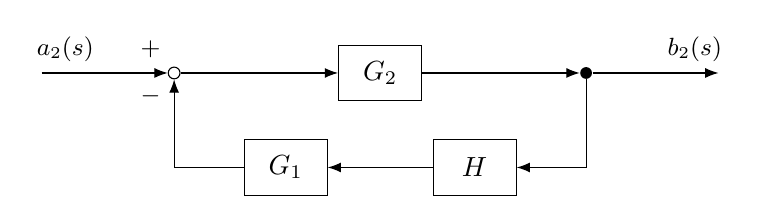
\begin{tikzpicture}[auto, node distance=1.6cm and 1.6cm, >=Latex]
    
      \node[input] (a1) {};
      \node[circle, draw, inner sep=1.5pt, right=of a1] (sum) {};
      \node[block, right=2.0cm of sum] (G2) {$G_2$};
      \node[circle, fill=black, inner sep=1.5pt, right=2.0cm of G2] (branch) {};
      \node[output, right=of branch] (b1) {};
    
      \node[block] at ($(G2)+(-1.2,-1.2)$) (G1) {$G_1$};
      \node[block] at ($(G2)+(1.2,-1.2)$) (H) {$H$};
    
      \draw[->] (a1) -- (sum);
      \draw[->] (sum) -- (G2);
      \draw[->] (G2) -- (branch);
      \draw[->] (branch) -- (b1);
    
      \draw[->] (branch) |- (H);
      \draw[->] (H) -- (G1);
      \draw[->] (G1) -| (sum);
    
      \node at ($(a1)+(0.3,0.3)$) {\small $a_2(s)$};
      \node at ($(b1)+(-0.3,0.3)$) {\small $b_2(s)$};
    
      \node at ($(sum)+(-0.3,0.3)$) {\small $+$};
      \node at ($(sum)+(-0.3,-0.3)$) {\small $-$};
    
    \end{tikzpicture}
  \end{center}

  \[
  b_2(s)=\frac{G_2}{1+G_1G_2H} \cdot a_2(s) \qquad \cdot \cdot \cdot (2)
  \]

  以上\((1),(2)\)より

  \begin{align*}
    b(s) & = b_1(s) + b_2(s)\\
        & = \frac{G_1 G_2 a_1(s)+G_2 a_2(s)}{1+G_1G_2H}
  \end{align*}



\end{tcolorbox}
% --------------- [45] --------------- 済
\begin{tcolorbox}[title={[45] \(\frac{b_1(s)}{a_1(s)}\),\(\frac{b_1(s)}{a_2(s)}\),\(\frac{b_2(s)}{a_1(s)}\),\(\frac{b_2(s)}{a_2(s)}\)を求めよ. 
  \vspace{-4mm}
  \begin{center}
    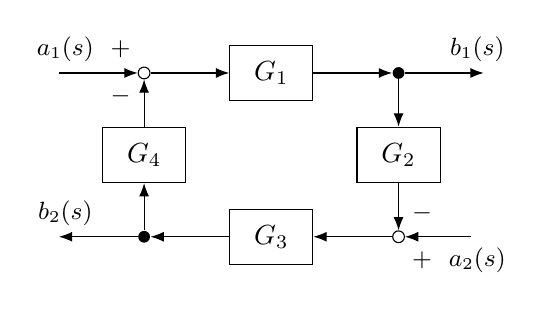
\begin{tikzpicture}[auto, node distance=0.8cm and 1.0cm, >=Latex]

% === 上段主系列(横) ===
\coordinate (input1);
\node[circle, draw, inner sep=1.5pt, right=of input1] (sum1) {};           % 合流点1
\node[block, right=of sum1] (G1) {$G_1$};                                  % G1
\node[circle, fill=black, inner sep=1.5pt, right=of G1] (branch1) {};      % 分岐点1
\coordinate[right=of branch1] (output1);                                   % 出力1(描画しない)

% === sum1の下:G4 → branch2(縦) ===
\node[block, below=0.6cm of sum1] (G4) {$G_4$};
\node[circle, fill=black, inner sep=1.5pt, below=0.6cm of G4] (branch2) {}; % 分岐点2

% === branch1の下:G2 → sum2(縦) ===
\node[block, below=0.6cm of branch1] (G2) {$G_2$};
\node[circle, draw, inner sep=1.5pt, below=0.6cm of G2] (sum2) {};          % 合流点2

% === 下段横系列:output2 ← branch2 ← G3 ← sum2 ← input2 ===
\coordinate[left=of branch2] (output2);
\node[block, right=of branch2] (G3) {$G_3$};
\coordinate[right=of G3] (sum2_right);
\coordinate[right=of sum2_right] (input2);

% === 経路 ===
\draw[->] (input1) -- (sum1);             % input1 → sum1
\draw[->] (sum1) -- (G1);                 % sum1 → G1
\draw[->] (G1) -- (branch1);              % G1 → branch1
\draw[->] (branch1) -- (output1);         % branch1 → output1

\draw[->] (input2) -- (sum2);       % input2 → sum2(右から)
\draw[->] (sum2_right) -- (G3);           % → G3
\draw[->] (G3) -- (branch2);              % G3 → branch2
\draw[->] (branch2) -- (output2);         % branch2 → output2

\draw[->] (branch1) -- (G2);              % 分岐1 → G2
\draw[->] (G2) -- (sum2);                 % G2 → 合流2

\draw[->] (branch2) -- (G4);              % 分岐2 → G4
\draw[->] (G4) -- (sum1);                 % G4 → 合流1

% === 加算記号 ===
\node at ($(sum1)+(-0.3,0.3)$) {\small $+$};
\node at ($(sum1)+(-0.3,-0.3)$) {\small $-$};
\node at ($(sum2)+(0.3,0.3)$) {\small $-$};
\node at ($(sum2)+(0.3,-0.3)$) {\small $+$};

% === その他記号 ===
\node at ($(sum1)+(-1.0,0.3)$) {\small $a_1(s)$};
\node at ($(branch1)+(1.0,0.3)$) {\small $b_1(s)$};
\node at ($(sum2)+(1.0,-0.3)$) {\small $a_2(s)$};
\node at ($(branch2)+(-1.0,0.3)$) {\small $b_2(s)$};

    \end{tikzpicture}
  \end{center}
  }]

  \(a_2(s)=0\)として
  \vspace{-2mm}
  \begin{center}
  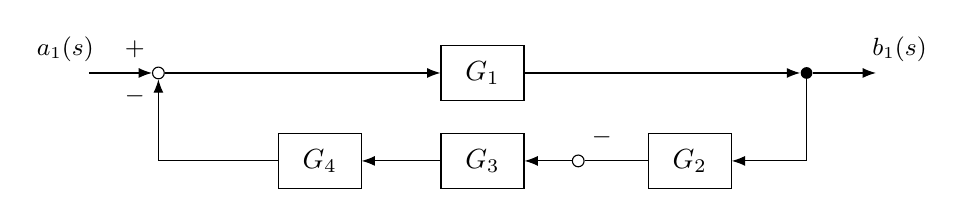
\begin{tikzpicture}[auto, node distance=0.8cm and 0.8cm, >=Latex]
  
    % --- 上段 ---
    \node[input] (a1) {};
    \node[circle, draw, inner sep=1.5pt, right=of a1] (sum1) {};
    \node[block, right=3.5cm of sum1] (G1) {$G_1$};
    \node[circle, fill=black, inner sep=1.5pt, right=3.5cm of G1] (branch) {};
    \node[output, right=of branch] (b1) {};
  
    % --- 下段 ---
    \node[block, below=0.4cm of G1] (G3) {$G_3$};
    \node[circle, draw, inner sep=1.5pt, right=0.6cm of G3] (sum2) {};
    \node[block, right=0.8cm of sum2] (G2) {$G_2$};
    \node[block, left=1.0cm of G3] (G4) {$G_4$};
  
    \draw[->] (a1) -- (sum1);
    \draw[->] (sum1) -- (G1);
    \draw[->] (G1) -- (branch);
    \draw[->] (branch) -- (b1);
  
    \draw[->] (branch) |- (G2);
    \draw[-] (G2) -- (sum2);
    \draw[->] (sum2) -- (G3);
    \draw[->] (G3) -- (G4);
    \draw[->] (G4) -| (sum1);
  
    % --- ラベル ---
    \node at ($(a1)+(-0.3,0.3)$) {\small $a_1(s)$};
    \node at ($(b1)+(0.3,0.3)$) {\small $b_1(s)$};
  
    % --- 加算記号 ---
    \node at ($(sum1)+(-0.3,0.3)$) {\small $+$};
    \node at ($(sum1)+(-0.3,-0.3)$) {\small $-$};
    \node at ($(sum2)+(0.3,0.3)$) {\small $-$};
  
  \end{tikzpicture}
  \end{center}

  \[
  \frac{b_1(s)}{a_1(s)}=\frac{1}{1-G_1 G_2 G_3 G_4}
  \]

  \begin{center}
    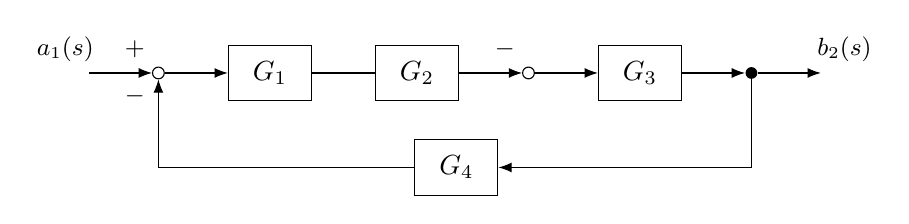
\begin{tikzpicture}[auto, node distance=1.6cm and 0.8cm, >=Latex]
  
      % 上段ノード
      \node[input] (a1) {};
      \node[circle, draw, inner sep=1.5pt, right=of a1] (sum1) {};
      \node[block, right=of sum1] (G1) {$G_1$};
      \node[block, right=of G1] (G2) {$G_2$};
      \node[circle, draw, inner sep=1.5pt, right=of G2] (sum2) {};
      \node[block, right=of sum2] (G3) {$G_3$};
      \node[circle, fill=black, inner sep=1.5pt, right=of G3] (branch) {};
      \node[output, right=of branch] (b2) {};
  
      % 下段ノード
      \node[block] at ($(G2)+(0.5,-1.2)$) (G4) {$G_4$};
  
      % 経路1:上段直線
      \draw[->] (a1) -- (sum1);
      \draw[->] (sum1) -- (G1);
      \draw[-] (G1) -- (G2);
      \draw[->] (G2) -- (sum2);
      \draw[->] (sum2) -- (G3);
      \draw[->] (G3) -- (branch);
      \draw[->] (branch) -- (b2);
  
      % 経路2:分岐 → G4 → sum1
      \draw[->] (branch) |- (G4);
      \draw[->] (G4) -| (sum1);
  
      % ラベル
      \node at ($(a1)+(-0.3,0.3)$) {\small $a_1(s)$};
      \node at ($(b2)+(0.3,0.3)$) {\small $b_2(s)$};
  
      % 加算記号
      \node at ($(sum1)+(-0.3,0.3)$) {\small $+$};
      \node at ($(sum1)+(-0.3,-0.3)$) {\small $-$};
      \node at ($(sum2)+(-0.3,0.3)$) {\small $-$};
  
    \end{tikzpicture}
  \end{center}

  \[
  \frac{b_1(s)}{a_1(s)}=\frac{1}{1-G_1 G_2 G_3 G_4}
  \]

  \(a_1(s)=0\)として
  \vspace{-2mm}
  \begin{center}
    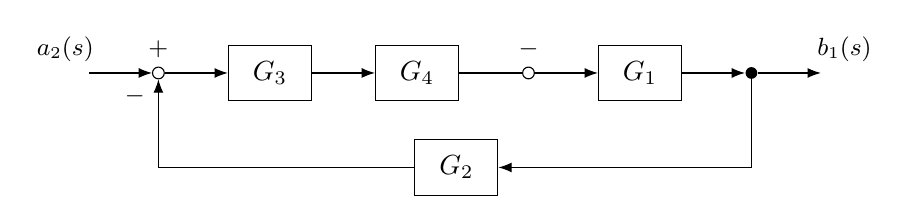
\begin{tikzpicture}[auto, node distance=1.6cm and 0.8cm, >=Latex]
  
      % 上段ノード
      \node[input] (a2) {};
      \node[circle, draw, inner sep=1.5pt, right=of a2] (sum2) {};
      \node[block, right=of sum2] (G3) {$G_3$};
      \node[block, right=of G3] (G4) {$G_4$};
      \node[circle, draw, inner sep=1.5pt, right=of G4] (sum1) {};
      \node[block, right=of sum1] (G1) {$G_1$};
      \node[circle, fill=black, inner sep=1.5pt, right=of G1] (branch) {};
      \node[output, right=of branch] (b1) {};
  
      % 下段ノード
      \node[block] at ($(G4)+(0.5,-1.2)$) (G2) {$G_2$};
  
      % 経路1(上段直線)
      \draw[->] (a2) -- (sum2);
      \draw[->] (sum2) -- (G3);
      \draw[->] (G3) -- (G4);
      \draw[-] (G4) -- (sum1);
      \draw[->] (sum1) -- (G1);
      \draw[->] (G1) -- (branch);
      \draw[->] (branch) -- (b1);
  
      % 経路2(分岐 → G2 → sum2)
      \draw[->] (branch) |- (G2);
      \draw[->] (G2) -| (sum2);
  
      % ラベル
      \node at ($(a2)+(-0.3,0.3)$) {\small $a_2(s)$};
      \node at ($(b1)+(0.3,0.3)$) {\small $b_1(s)$};
  
      % 加算記号
      \node at ($(sum2)+(0,0.3)$) {\small $+$};
      \node at ($(sum2)+(-0.3,-0.3)$) {\small $-$};
      \node at ($(sum1)+(0,0.3)$) {\small $-$};
  
    \end{tikzpicture}
  \end{center}

  \[
  \frac{b_1(s)}{a_1(s)}=\frac{1}{1-G_1 G_2 G_3 G_4}
  \]

  \begin{center}
    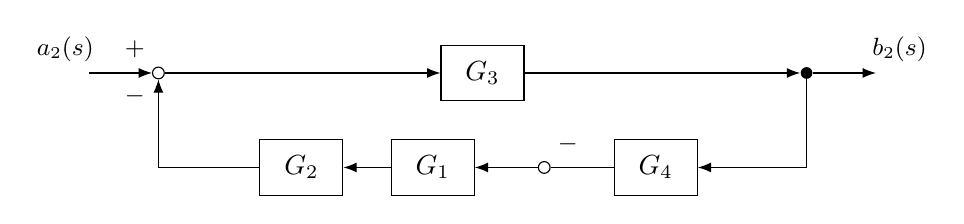
\begin{tikzpicture}[auto, node distance=0.8cm and 0.8cm, >=Latex]
  
      % 上段:a2 → sum2 → G3 → branch → b2
      \node[input] (a2) {};
      \node[circle, draw, inner sep=1.5pt, right=of a2] (sum2) {};
      \node[block, right=3.5cm of sum2] (G3) {$G_3$};
      \node[circle, fill=black, inner sep=1.5pt, right=3.5cm of G3] (branch) {};
      \node[output, right=of branch] (b2) {};
  
      % 下段:G4 → sum1 → G1 → G2 → sum2
      \node[block] at ($(G3)+(2.2,-1.2)$) (G4) {$G_4$};
      \node[circle, draw, inner sep=1.5pt, left=0.8cm of G4] (sum1) {};
      \node[block, left=0.8cm of sum1] (G1) {$G_1$};
      \node[block, left=0.6cm of G1] (G2) {$G_2$};
  
      % 経路:上段
      \draw[->] (a2) -- (sum2);
      \draw[->] (sum2) -- (G3);
      \draw[->] (G3) -- (branch);
      \draw[->] (branch) -- (b2);
  
      % 経路:フィードバックルート
      \draw[->] (branch) |- (G4);
      \draw[-] (G4) -- (sum1);
      \draw[->] (sum1) -- (G1);
      \draw[->] (G1) -- (G2);
      \draw[->] (G2) -| (sum2);
  
      % ラベル
      \node at ($(a2)+(-0.3,0.3)$) {\small $a_2(s)$};
      \node at ($(b2)+(0.3,0.3)$) {\small $b_2(s)$};
  
      % 加算記号
      \node at ($(sum2)+(-0.3,0.3)$) {\small $+$};
      \node at ($(sum2)+(-0.3,-0.3)$) {\small $-$};
      \node at ($(sum1)+(0.3,0.3)$) {\small $-$};

    \end{tikzpicture}
  \end{center} 

  \[
  \frac{b_1(s)}{a_1(s)}=\frac{1}{1-G_1 G_2 G_3 G_4}
  \]



\end{tcolorbox}
% --------------- [46] --------------- 済
\begin{tcolorbox}[title={[46] ブロック線図を簡単にせよ.
  \vspace{-12mm}
  \begin{center}
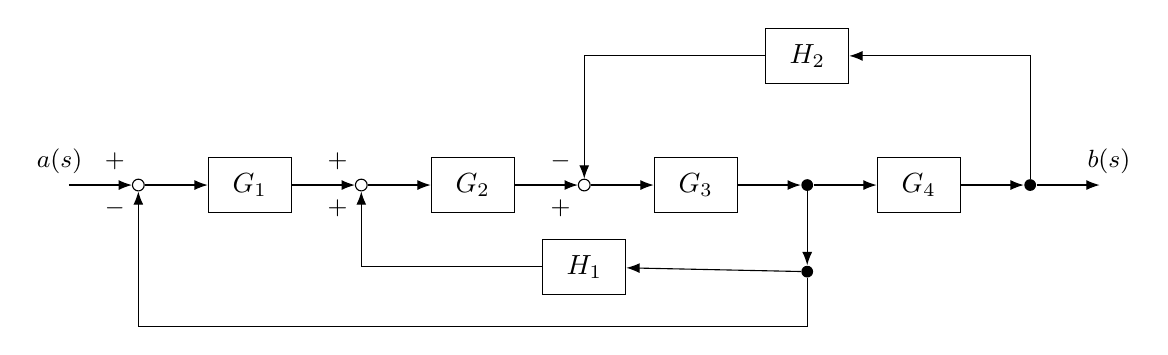
\begin{tikzpicture}[auto, node distance=0.6cm and 0.8cm, >=Latex]

  % --- 主系列ノード(横並び) ---
  \coordinate (input);
  \node[circle, draw, inner sep=1.5pt, right=of input] (sum1) {};        % 合流1
  \node[block, right=of sum1] (G1) {$G_1$};                               % G1
  \node[circle, draw, inner sep=1.5pt, right=of G1] (sum2) {};           % 合流2
  \node[block, right=of sum2] (G2) {$G_2$};                               % G2
  \node[circle, draw, inner sep=1.5pt, right=of G2] (sum3) {};           % 合流3
  \node[block, right=of sum3] (G3) {$G_3$};                               % G3
  \node[circle, fill=black, inner sep=1.5pt, right=of G3] (branch1) {};  % 分岐1
  \node[block, right=of branch1] (G4) {$G_4$};                            % G4
  \node[circle, fill=black, inner sep=1.5pt, right=of G4] (branch2) {};  % 分岐2
  \coordinate[right=of branch2] (output);

  % --- 上下ノード配置 ---
  \node[block, above=1.2cm of branch1] (H2) {$H_2$};                      % H2(分岐1の上)
  \node[block, below=of sum3] (H1) {$H_1$};                         % H1(合流3の下)
  \node[circle, fill=black, inner sep=1.5pt] at ($(branch1)+(0,-1.1)$) (branch3) {};% 分岐3(分岐1の下)

  % --- 経路①: input → ... → output ---
  \draw[->] (input) -- (sum1);
  \draw[->] (sum1) -- (G1);
  \draw[->] (G1) -- (sum2);
  \draw[->] (sum2) -- (G2);
  \draw[->] (G2) -- (sum3);
  \draw[->] (sum3) -- (G3);
  \draw[->] (G3) -- (branch1);
  \draw[->] (branch1) -- (G4);
  \draw[->] (G4) -- (branch2);
  \draw[->] (branch2) -- (output);

  % --- 経路②: 分岐2 → H2 → 合流3 ---
  \draw[->] (branch2) |- (H2);
  \draw[->] (H2) -| (sum3);

  % --- 経路③: 分岐1 → 分岐3 → H1 → 合流2 ---
  \draw[->] (branch1) -- (branch3);
  \draw[->] (branch3) -- (H1);
  \draw[->] (H1) -| (sum2);

  % --- 経路④: 分岐3 → ↓←↑ → 合流1 ---
  \coordinate (pivot) at ($(sum1)+(0,-1.8)$); % 合流点1の下
  \draw[->] (branch3) |-(pivot) -- (sum1);

  % --- 加算記号配置 ---
  \node at ($(sum1)+(-0.3,0.3)$) {\small $+$};
  \node at ($(sum1)+(-0.3,-0.3)$) {\small $-$};
  \node at ($(sum2)+(-0.3,0.3)$) {\small $+$};
  \node at ($(sum2)+(-0.3,-0.3)$) {\small $+$};
  \node at ($(sum3)+(-0.3,0.3)$) {\small $-$};
  \node at ($(sum3)+(-0.3,-0.3)$) {\small $+$};

  % --- その他記号配置 ---
  \node at ($(sum1)+(-1.0,0.3)$) {\small $a(s)$};
  \node at ($(branch2)+(1.0,0.3)$) {\small $b(s)$};

\end{tikzpicture}
  \end{center}
  \vspace{2mm}
  }]

  \begin{center}
    \begin{tikzpicture}[auto, node distance=0.4cm and 0.6cm, >=Latex]
    
      % === 中段(主系列) ===
      \node[input] (a) {};
      \node[circle, draw, inner sep=1.5pt, right=of a] (sum1) {};
      \node[block, right=of sum1] (G1) {$G_1$};
      \node[circle, draw, inner sep=1.5pt, right=of G1] (sum2) {};
      \node[block, right=of sum2] (G2) {$G_2$};
      \node[circle, draw, inner sep=1.5pt, right=of G2] (sum3) {};
      \node[block, right=1.6cm of sum3] (G3) {$G_3$};
      \node[circle, fill=black, inner sep=1.5pt, right=1.6cm of G3] (branch1) {};
      \node[block, right=0.8cm of branch1] (H4) {$G_4$};
      \node[output, right=of H4] (b) {};
    
      % === 上段(G4→H2) ===
      \node[block] at ($(branch1)+(-1.4,1.6)$) (G4) {$G_4$};
      \node[block, left=0.6cm of G4] (H2) {$H_2$};
    
      % === 下段(H1) ===
      \node[block] at ($(sum3)+(0,-1.6)$) (H1) {$H_1$};
    
      % === 経路(主系列) ===
      \draw[->] (a) -- (sum1);
      \draw[->] (sum1) -- (G1);
      \draw[->] (G1) -- (sum2);
      \draw[->] (sum2) -- (G2);
      \draw[->] (G2) -- (sum3);
      \draw[->] (sum3) -- (G3);
      \draw[->] (G3) -- (branch1);
      \draw[->] (branch1) -- (H4);
      \draw[->] (H4) -- (b);
    
      % === 経路:branch1 → G4 → H2 → sum3(上ループ)===
      \draw[->] (branch1) |- (G4);
      \draw[->] (G4) -- (H2);
      \draw[->] (H2) -| (sum3);
    
      % === 経路:branch1 → H1 → sum2(下ループ)===
      \draw[->] (branch1) |- (H1);
      \draw[->] (H1) -| (sum2);
    
      % === 経路:branch1 → sum1(フィードバック) ===
      \coordinate (pivot) at ($(sum1)+(0,-2.4)$);
      \draw[->] (branch1) |- (pivot) -- (sum1);
    
      % === ラベル ===
      \node at ($(a)+(-0.3,0.3)$) {\small $a(s)$};
      \node at ($(b)+(0.3,0.3)$) {\small $b(s)$};
    
      % === 加算記号 ===
      \node at ($(sum1)+(-0.3,0.3)$) {\small $+$};
      \node at ($(sum1)+(-0.3,-0.3)$) {\small $-$};
      \node at ($(sum2)+(-0.3,0.3)$) {\small $+$};
      \node at ($(sum2)+(-0.3,-0.3)$) {\small $+$};
      \node at ($(sum3)+(-0.3,0.3)$) {\small $-$};
      \node at ($(sum3)+(-0.3,-0.3)$) {\small $+$};
    
    \end{tikzpicture}

    \vspace{2mm}
    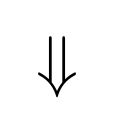
\begin{tikzpicture}
      \node {\Huge$\Downarrow$};
    \end{tikzpicture}
    \vspace{2mm}


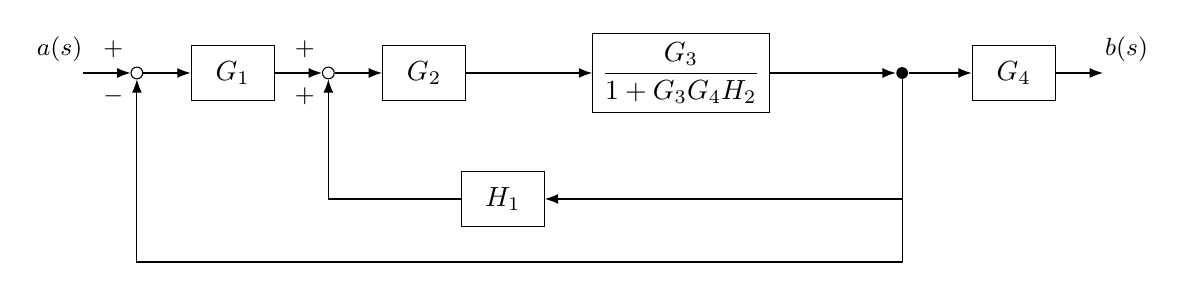
\begin{tikzpicture}[auto, node distance=0.4cm and 0.6cm, >=Latex]

  % 中段(主系列)
  \node[input] (a) {};
  \node[circle, draw, inner sep=1.5pt, right=of a] (sum1) {};
  \node[block, right=of sum1] (G1) {$G_1$};
  \node[circle, draw, inner sep=1.5pt, right=of G1] (sum2) {};
  \node[block, right=of sum2] (G2) {$G_2$};
  \node[block, right=1.6cm of G2] (G3combo) {$\dfrac{G_3}{1+G_3 G_4 H_2}$};
  \node[circle, fill=black, inner sep=1.5pt, right=1.6cm of G3combo] (branch1) {};
  \node[block, right=0.8cm of branch1] (G4) {$G_4$};
  \node[output, right=of G4] (b) {};

  % 下段:H1
  \node[block] at ($(G2)+(1.0,-1.6)$) (H1) {$H_1$};

  % 経路(主系列)
  \draw[->] (a) -- (sum1);
  \draw[->] (sum1) -- (G1);
  \draw[->] (G1) -- (sum2);
  \draw[->] (sum2) -- (G2);
  \draw[->] (G2) -- (G3combo);
  \draw[->] (G3combo) -- (branch1);
  \draw[->] (branch1) -- (G4);
  \draw[->] (G4) -- (b);

  % 下段ループ
  \draw[->] (branch1) |- (H1);
  \draw[->] (H1) -| (sum2);

  % フィードバック(sum1へ)
  \coordinate (pivot) at ($(sum1)+(0,-2.4)$);
  \draw[->] (branch1) |- (pivot) -- (sum1);

  % ラベル
  \node at ($(a)+(-0.3,0.3)$) {\small $a(s)$};
  \node at ($(b)+(0.3,0.3)$) {\small $b(s)$};

  % 加算記号
  \node at ($(sum1)+(-0.3,0.3)$) {\small $+$};
  \node at ($(sum1)+(-0.3,-0.3)$) {\small $-$};
  \node at ($(sum2)+(-0.3,0.3)$) {\small $+$};
  \node at ($(sum2)+(-0.3,-0.3)$) {\small $+$};

\end{tikzpicture}

    \vspace{2mm}
    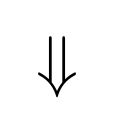
\begin{tikzpicture}
      \node {\Huge$\Downarrow$};
    \end{tikzpicture}
    \vspace{2mm}

    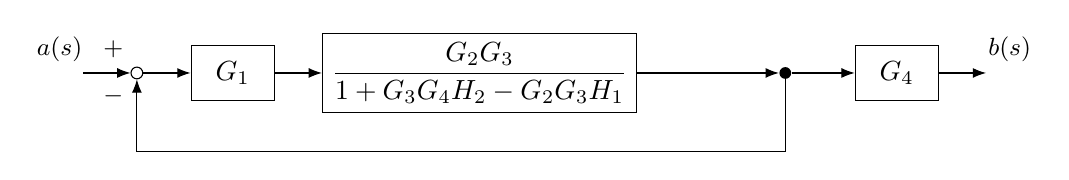
\begin{tikzpicture}[auto, node distance=0.4cm and 0.6cm, >=Latex]
    
      % ノード配置
      \node[input] (a) {};
      \node[circle, draw, inner sep=1.5pt, right=of a] (sum1) {};
      \node[block, right=of sum1] (G1) {$G_1$};
      \node[block, right=of G1] (G2G3combo) 
        {$\dfrac{G_2 G_3}{1 + G_3 G_4 H_2 - G_2 G_3 H_1}$};
      \node[circle, fill=black, inner sep=1.5pt, right=1.8cm of G2G3combo] (branch1) {};
      \node[block, right=0.8cm of branch1] (G4final) {$G_4$};
      \node[output, right=of G4final] (b) {};
    
      % 経路
      \draw[->] (a) -- (sum1);
      \draw[->] (sum1) -- (G1);
      \draw[->] (G1) -- (G2G3combo);
      \draw[->] (G2G3combo) -- (branch1);
      \draw[->] (branch1) -- (G4final);
      \draw[->] (G4final) -- (b);
    
      % フィードバック:branch1 → sum1 (最終帰還)
      \coordinate (pivot1) at ($(sum1)+(0,-1.0)$);
      \draw[->] (branch1) |- (pivot1) -- (sum1);
    
      % ラベル
      \node at ($(a)+(-0.3,0.3)$) {\small $a(s)$};
      \node at ($(b)+(0.3,0.3)$) {\small $b(s)$};
      \node at ($(sum1)+(-0.3,0.3)$) {\small $+$};
      \node at ($(sum1)+(-0.3,-0.3)$) {\small $-$};
    
    \end{tikzpicture}

    \vspace{2mm}
    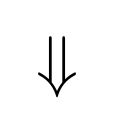
\begin{tikzpicture}
      \node {\Huge$\Downarrow$};
    \end{tikzpicture}
    \vspace{2mm}


    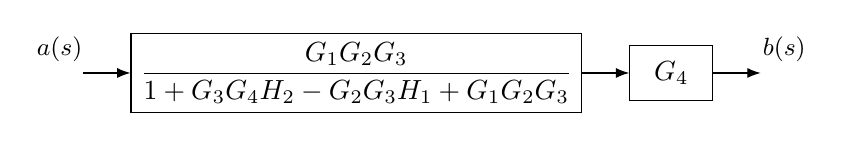
\begin{tikzpicture}[auto, node distance=0.4cm and 0.6cm, >=Latex]
    
      % ノード配置
      \node[input] (a) {};
      \node[block, right=of a] (core) 
        {$\dfrac{G_1 G_2 G_3}{1 + G_3 G_4 H_2 - G_2 G_3 H_1 + G_1 G_2 G_3}$};
      \node[block, right=of core] (G4) {$G_4$};
      \node[output, right=of G4] (b) {};
    
      % 経路
      \draw[->] (a) -- (core);
      \draw[->] (core) -- (G4);
      \draw[->] (G4) -- (b);
    
      % ラベル
      \node at ($(a)+(-0.3,0.3)$) {\small $a(s)$};
      \node at ($(b)+(0.3,0.3)$) {\small $b(s)$};
    
    \end{tikzpicture}

    \vspace{2mm}
    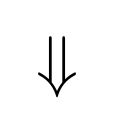
\begin{tikzpicture}
      \node {\Huge$\Downarrow$};
    \end{tikzpicture}
    \vspace{2mm}

    \vspace{2mm}
    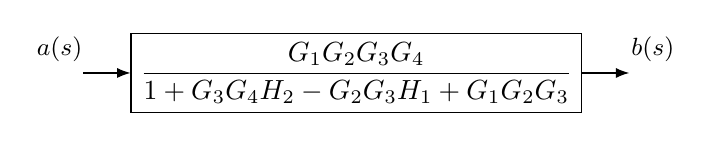
\begin{tikzpicture}[auto, node distance=0.4cm and 0.6cm, >=Latex]
    
      \node[input] (a) {};
      \node[block, right=of a] (Gtotal) 
        {$\dfrac{G_1 G_2 G_3 G_4}{1 + G_3 G_4 H_2 - G_2 G_3 H_1 + G_1 G_2 G_3}$};
      \node[output, right=of Gtotal] (b) {};
    
      \draw[->] (a) -- (Gtotal);
      \draw[->] (Gtotal) -- (b);
    
      \node at ($(a)+(-0.3,0.3)$) {\small $a(s)$};
      \node at ($(b)+(0.3,0.3)$) {\small $b(s)$};
    
    \end{tikzpicture}
  \end{center}







\end{tcolorbox}
% --------------- [47] --------------- 済
\begin{tcolorbox}[title={[47] ブロック線図を簡単にせよ. 
  \begin{center}
    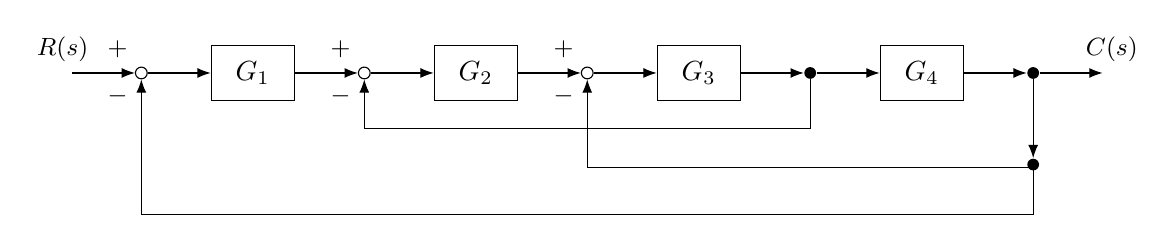
\begin{tikzpicture}[auto, node distance=0.8cm and 0.8cm, >=Latex]
      % --- 横並びの主系列ノード ---
      \node at (0,0) (input) {};
      \node[circle, draw, inner sep=1.5pt, right=of input] (sum1) {};           % 合流点1
      \node[block, right=of sum1] (G1) {$G_1$};
      \node[circle, draw, inner sep=1.5pt, right=of G1] (sum2) {};             % 合流点2
      \node[block, right=of sum2] (G2) {$G_2$};
      \node[circle, draw, inner sep=1.5pt, right=of G2] (sum3) {};             % 合流点3
      \node[block, right=of sum3] (G3) {$G_3$};
      \node[circle, fill=black, inner sep=1.5pt, right=of G3] (branch1) {};    % 分岐点1
      \node[block, right=of branch1] (G4) {$G_4$};
      \node[circle, fill=black, inner sep=1.5pt, right=of G4] (branch2) {};    % 分岐点2
      \node[right=of branch2] (output) {};
    
      % --- 分岐点3(branch2の下) ---
      \node[circle, fill=black, inner sep=1.5pt, below=1.0cm of branch2] (branch3) {};
    
      % === 主系列経路 ===
      \draw[->] (input) -- (sum1);
      \draw[->] (sum1) -- (G1);
      \draw[->] (G1) -- (sum2);
      \draw[->] (sum2) -- (G2);
      \draw[->] (G2) -- (sum3);
      \draw[->] (sum3) -- (G3);
      \draw[->] (G3) -- (branch1);
      \draw[->] (branch1) -- (G4);
      \draw[->] (G4) -- (branch2);
      \draw[->] (branch2) -- (output);
    
      % === 追加経路 ===
        % 分岐1 → 合流2(カクカク経路:下→左→上)
        \coordinate (pivot12) at ($(sum2)+(0,-0.7)$); 
        \draw[->] (branch1) |- (pivot12) -| (sum2);
    
        % 分岐2 → 分岐3(真下に新ノード) ←既に実装済
        \draw[->] (branch2) -- (branch3);
    
        % 分岐3 → 合流3(カクカク経路:下→左→上)
        \coordinate (pivot33) at ($(sum3)+(0,-1.2)$);
        \draw[->] (branch3) |- (pivot33) -| (sum3);              
    
      % 分岐3 → 合流1(カクカク:下→左→上、1本の矢印で)
      \coordinate (pivot) at ($(sum1)+(0,-1.8)$);
      \draw[->] (branch3) |- (pivot) -| (sum1);
    
    
      % --- 加算記号配置 ---
      \node at ($(sum1)+(-0.3,0.3)$) {\small $+$};
      \node at ($(sum1)+(-0.3,-0.3)$) {\small $-$};
      \node at ($(sum2)+(-0.3,0.3)$) {\small $+$};
      \node at ($(sum2)+(-0.3,-0.3)$) {\small $-$};
      \node at ($(sum3)+(-0.3,0.3)$) {\small $+$};
      \node at ($(sum3)+(-0.3,-0.3)$) {\small $-$};
    
      \node at ($(sum1)+(-1.0,0.3)$) {\small $R(s)$};
      \node at ($(branch2)+(1.0,0.3)$) {\small $C(s)$};
    
  \end{tikzpicture}
  \end{center}
  \vspace{2mm}
  }]

  \begin{center}
    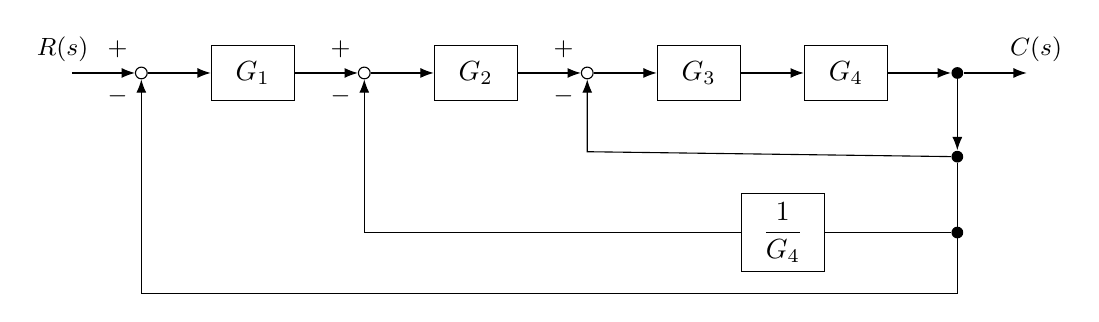
\begin{tikzpicture}[auto, node distance=0.8cm and 0.8cm, >=Latex]
      % --- 横並びの主系列ノード ---
      \node at (0,0) (input) {};
      \node[circle, draw, inner sep=1.5pt, right=of input] (sum1) {};           % 合流点1
      \node[block, right=of sum1] (G1) {$G_1$};
      \node[circle, draw, inner sep=1.5pt, right=of G1] (sum2) {};             % 合流点2
      \node[block, right=of sum2] (G2) {$G_2$};
      \node[circle, draw, inner sep=1.5pt, right=of G2] (sum3) {};             % 合流点3
      \node[block, right=of sum3] (G3) {$G_3$};
      \node[block, right=of G3] (G4) {$G_4$};
      \node[circle, fill=black, inner sep=1.5pt, right=of G4] (branch2) {};    % 分岐点2
      \node[right=of branch2] (output) {};
    
      % --- 分岐点3(branch2の下) ---
      \node[circle, fill=black, inner sep=1.5pt, below=0.9cm of branch2] (branch3) {};
      
      % --- 分岐点1(branch3の下) ---
      \node[circle, fill=black, inner sep=1.5pt, below=of branch3] (branch1) {};
      \node[block, left=1.6cm of branch1] (G4') {$\dfrac{1}{G_4}$};
    
      % === 主系列経路 ===
      \draw[->] (input) -- (sum1);
      \draw[->] (sum1) -- (G1);
      \draw[->] (G1) -- (sum2);
      \draw[->] (sum2) -- (G2);
      \draw[->] (G2) -- (sum3);
      \draw[->] (sum3) -- (G3);
      \draw[->] (G3) -- (G4);
      \draw[->] (G4) -- (branch2);
      \draw[->] (branch2) -- (output);
    
      % === 追加経路 ===
        % 分岐1 → 合流2(カクカク経路:上→左→上)
        \draw[->] (branch1) -- (G4') -| (sum2);
    
        % 分岐2 → 分岐3(真下に新ノード)
        \draw[->] (branch2) -- (branch3);
    
        % 分岐3 → 合流3(カクカク経路:下→左→上)
        \coordinate (pivot33) at ($(sum3)+(0,-1.0)$);
        \draw[->] (branch3) -- (pivot33) -| (sum3);              
    
        % 分岐3 → 合流1(カクカク:下→左→上、1本の矢印で)
        \coordinate (pivot) at ($(sum1)+(0,-2.8)$);
        \draw[->] (branch3) |- (pivot) -| (sum1);
    
      % --- 加算記号配置 ---
      \node at ($(sum1)+(-0.3,0.3)$) {\small $+$};
      \node at ($(sum1)+(-0.3,-0.3)$) {\small $-$};
      \node at ($(sum2)+(-0.3,0.3)$) {\small $+$};
      \node at ($(sum2)+(-0.3,-0.3)$) {\small $-$};
      \node at ($(sum3)+(-0.3,0.3)$) {\small $+$};
      \node at ($(sum3)+(-0.3,-0.3)$) {\small $-$};
    
      \node at ($(sum1)+(-1.0,0.3)$) {\small $R(s)$};
      \node at ($(branch2)+(1.0,0.3)$) {\small $C(s)$};
    
    \end{tikzpicture}


  \vspace{2mm}
    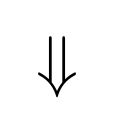
\begin{tikzpicture}
      \node {\Huge$\Downarrow$};
    \end{tikzpicture}
  \vspace{2mm}



  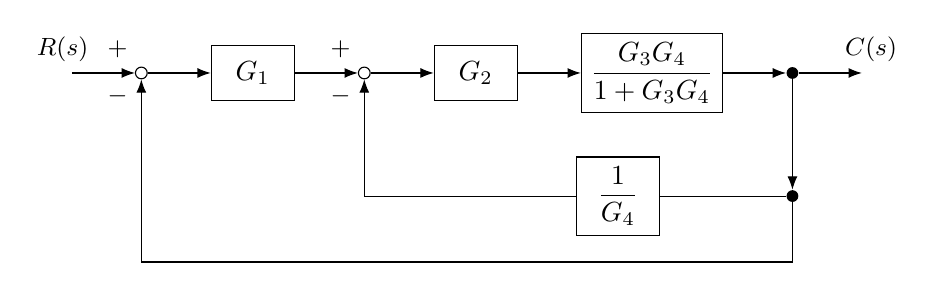
\begin{tikzpicture}[auto, node distance=0.8cm and 0.8cm, >=Latex]
    % --- 横並びの主系列ノード ---
    \node at (0,0) (input) {};
    \node[circle, draw, inner sep=1.5pt, right=of input] (sum1) {};           % 合流点1
    \node[block, right=of sum1] (G1) {$G_1$};
    \node[circle, draw, inner sep=1.5pt, right=of G1] (sum2) {};             % 合流点2
    \node[block, right=of sum2] (G2) {$G_2$};           % 合流点3
    \node[block, right=of G2] (G34) {$\dfrac{G_3 G_4}{1 + G_3 G_4}$};       % 合成ブロック
    \node[circle, fill=black, inner sep=1.5pt, right=of G34] (branch2) {};   % 分岐点2
    \node[right=of branch2] (output) {};
    
    % --- 分岐点1(branch3の下) ---
    \node[circle, fill=black, inner sep=1.5pt, below=1.4cm of branch2] (branch1) {};
    \node[block, left=1.6cm of branch1] (G4inv) {$\dfrac{1}{G_4}$};
  
    % === 主系列経路 ===
    \draw[->] (input) -- (sum1);
    \draw[->] (sum1) -- (G1);
    \draw[->] (G1) -- (sum2);
    \draw[->] (sum2) -- (G2);
    \draw[->] (G2)  -- (G34);
    \draw[->] (G34) -- (branch2);
    \draw[->] (branch2) -- (output);
  
    % === 追加経路 ===
      % 分岐1 → 合流2(カクカク経路:上→左→上)
      \draw[->] (branch1) -- (G4inv) -| (sum2);
  
      % 分岐2 → 分岐3(真下に新ノード)
      \draw[->] (branch2) -- (branch1);
  
      % 分岐3 → 合流1(カクカク:下→左→上、1本の矢印で)
      \coordinate (pivot) at ($(sum1)+(0,-2.4)$);
      \draw[->] (branch1) |- (pivot) -| (sum1);
  
    % --- 加算記号配置 ---
    \node at ($(sum1)+(-0.3,0.3)$) {\small $+$};
    \node at ($(sum1)+(-0.3,-0.3)$) {\small $-$};
    \node at ($(sum2)+(-0.3,0.3)$) {\small $+$};
    \node at ($(sum2)+(-0.3,-0.3)$) {\small $-$};

  
    \node at ($(sum1)+(-1.0,0.3)$) {\small $R(s)$};
    \node at ($(branch2)+(1.0,0.3)$) {\small $C(s)$};
  
  \end{tikzpicture}

  \vspace{2mm}
    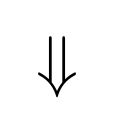
\begin{tikzpicture}
      \node {\Huge$\Downarrow$};
    \end{tikzpicture}
  \vspace{2mm}


  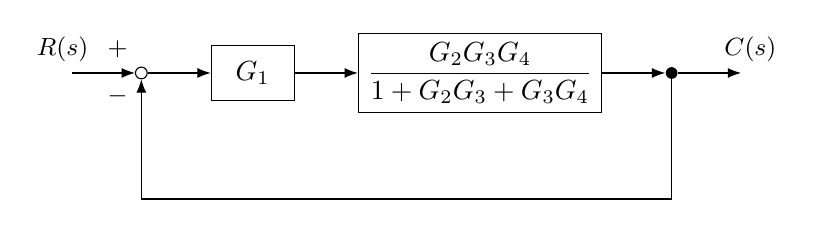
\begin{tikzpicture}[auto, node distance=0.8cm and 0.8cm, >=Latex]
    % --- 横並びの主系列ノード ---
    \node at (0,0) (input) {};
    \node[circle, draw, inner sep=1.5pt, right=of input] (sum1) {};                   % 合流点1
    \node[block, right=of sum1] (G1) {$G_1$};
    \node[block, right=of G1] (G234) {$\dfrac{G_2 G_3 G_4}{1 + G_2 G_3 + G_3 G_4}$};             % 合成ブロック
    \node[circle, fill=black, inner sep=1.5pt, right=of G234] (branch2) {};           % 分岐点2
    \node[right=of branch2] (output) {};
  
    % === 主系列経路 ===
    \draw[->] (input) -- (sum1);
    \draw[->] (sum1) -- (G1);
    \draw[->] (G1) -- (G234);
    \draw[->] (G234) -- (branch2);
    \draw[->] (branch2) -- (output);
  
    % === フィードバック(branch2 → sum1) ===
    \coordinate (pivot) at ($(sum1)+(0,-1.6)$);
    \draw[->] (branch2) |- (pivot) -| (sum1);
  
    % --- 加算記号配置 ---
    \node at ($(sum1)+(-0.3,0.3)$) {\small $+$};
    \node at ($(sum1)+(-0.3,-0.3)$) {\small $-$};
  
    \node at ($(sum1)+(-1.0,0.3)$) {\small $R(s)$};
    \node at ($(branch2)+(1.0,0.3)$) {\small $C(s)$};
  
  \end{tikzpicture}

  \vspace{2mm}
    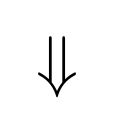
\begin{tikzpicture}
      \node {\Huge$\Downarrow$};
    \end{tikzpicture}
  \vspace{2mm}



  \begin{tikzpicture}[auto, node distance=1.0cm and 1.5cm, >=Latex]
      % --- 入出力とブロック ---
      \node at (0,0) (input) {};
      \node[block, right=of input] (Gfinal) {$\dfrac{G_1 G_2 G_3 G_4}{1 + G_2 G_3 + G_3 G_4  + G_1 G_2 G_3 G_4}$};
      \node[right=of Gfinal] (output) {};
    
      % --- 矢印 ---
      \draw[->] (input) -- (Gfinal);
      \draw[->] (Gfinal) -- (output);
    
      % --- ラベル ---
      \node at ($(sum1)+(-1.0,0.3)$) {\small $R(s)$};
      \node at ($(branch2)+(1.0,0.3)$) {\small $C(s)$};
  \end{tikzpicture}


\end{center}

\end{tcolorbox}
% --------------- [48] --------------- 済
\begin{tcolorbox}[title={[48] ブロック線図を簡単にせよ. 
  \begin{center}
    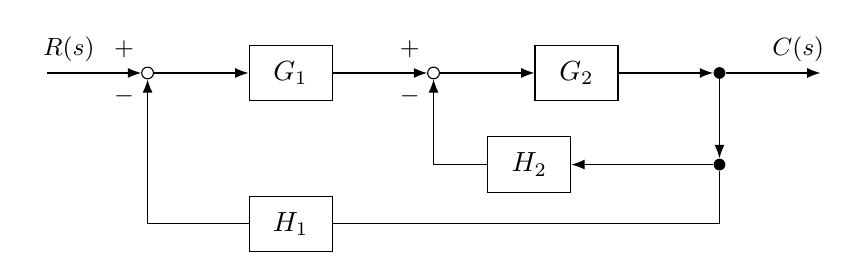
\begin{tikzpicture}[auto, node distance=0.8cm and 1.2cm, >=Latex]

      % --- 横並びの主系列ノード ---
      \node at (0,0) (input) {};
      \node[circle, draw, inner sep=1.5pt, right=of input] (sum1) {};           % 合流点1
      \node[block, right=of sum1] (G1) {$G_1$};
      \node[circle, draw, inner sep=1.5pt, right=of G1] (sum2) {};             % 合流点2
      \node[block, right=of sum2] (G2) {$G_2$};
      \node[circle, fill=black, inner sep=1.5pt, right=of G2] (branch1) {};    % 分岐点1
      \node[right=of branch1] (output) {};                                     % 出力
  
      % --- 下部ノード配置 ---
      \node[circle, fill=black, inner sep=1.5pt, below=1.0cm of branch1] (branch2) {}; % 分岐点2
      \node[block, left=1.8cm of branch2] (H2) {$H_2$};                                 % H2
      \node[block, below=1.2cm of G1] (H1) {$H_1$};                                     % H1(H2より下)
  
      % === 主系列経路 ===
      \draw[->] (input) -- (sum1);
      \draw[->] (sum1) -- (G1);
      \draw[->] (G1) -- (sum2);
      \draw[->] (sum2) -- (G2);
      \draw[->] (G2) -- (branch1);
      \draw[->] (branch1) -- (output);
  
      % === 追加経路 ===
      % 分岐1 → 分岐2(真下)
      \draw[->] (branch1) -- (branch2);
  
      % 分岐2 → H2 → 合流点2(カクカク:左→上→右)
  
      \draw[->] (branch2) -- (H2);
      \draw[->] (H2) -| (sum2);
  
      % 分岐2 → H1 → 合流点1(カクカク:下→左→上)
      \draw[->] (branch2) |- (H1) -| (sum1);
  
      % --- 加算記号配置 ---
      \node at ($(sum1)+(-0.3,0.3)$) {\small $+$};
      \node at ($(sum1)+(-0.3,-0.3)$) {\small $-$};
      \node at ($(sum2)+(-0.3,0.3)$) {\small $+$};
      \node at ($(sum2)+(-0.3,-0.3)$) {\small $-$};
  
      % --- その他記号配置 ---
      \node at ($(sum1)+(-1.0,0.3)$) {\small $R(s)$};
      \node at ($(branch1)+(1.0,0.3)$) {\small $C(s)$};
  
  \end{tikzpicture}
  \end{center}
  \vspace{2mm}
  }]

  \begin{center}
    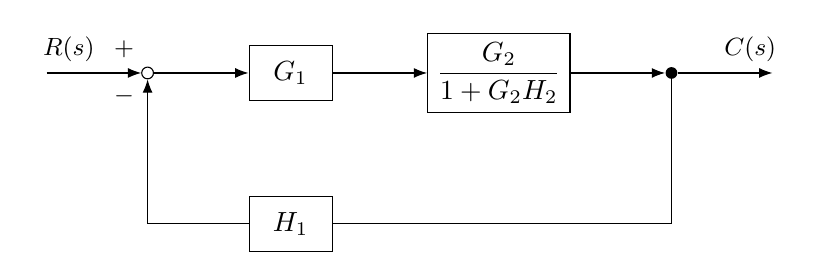
\begin{tikzpicture}[auto, node distance=0.8cm and 1.2cm, >=Latex]
    
      % --- 横並びの主系列ノード ---
      \node at (0,0) (input) {};
      \node[circle, draw, inner sep=1.5pt, right=of input] (sum1) {};                  % 合流点1
      \node[block, right=of sum1] (G1) {$G_1$};
      \node[block, right=of G1] (G2H2) {$\dfrac{G_2}{1 + G_2 H_2}$};                   % フィードバック合成済ブロック
      \node[circle, fill=black, inner sep=1.5pt, right=of G2H2] (branch1) {};         % 分岐点1
      \node[right=of branch1] (output) {};                                            % 出力
    
      % --- 下部ノード(H1のみ) ---
      \node[block, below=1.2cm of G1] (H1) {$H_1$};
    
      % === 主系列経路 ===
      \draw[->] (input) -- (sum1);
      \draw[->] (sum1) -- (G1);
      \draw[->] (G1) -- (G2H2);
      \draw[->] (G2H2) -- (branch1);
      \draw[->] (branch1) -- (output);
    
      % === フィードバック H1 のみ ===
      \draw[->] (branch1) |- (H1) -| (sum1);
    
      % --- 加算記号配置 ---
      \node at ($(sum1)+(-0.3,0.3)$) {\small $+$};
      \node at ($(sum1)+(-0.3,-0.3)$) {\small $-$};
    
      % --- ラベル配置 ---
      \node at ($(sum1)+(-1.0,0.3)$) {\small $R(s)$};
      \node at ($(branch1)+(1.0,0.3)$) {\small $C(s)$};
    
    \end{tikzpicture}

    \vspace{2mm}
    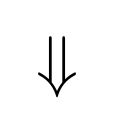
\begin{tikzpicture}
      \node {\Huge$\Downarrow$};
    \end{tikzpicture}
  \vspace{2mm}

    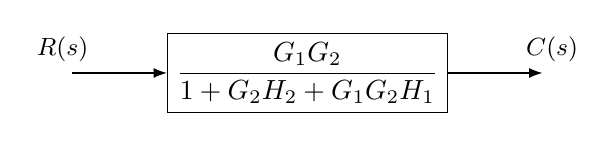
\begin{tikzpicture}[auto, node distance=1.5cm and 1.2cm, >=Latex]
    
      % --- ノード構成 ---
      \node at (0,0) (input) {};
      \node[block, right=of input] (Gfinal) {$\dfrac{G_1 G_2}{1 + G_2 H_2 + G_1 G_2 H_1}$};
      \node[right=of Gfinal] (output) {};
    
      % --- 主系列矢印 ---
      \draw[->] (input) -- (Gfinal);
      \draw[->] (Gfinal) -- (output);
    
      % --- 入出力ラベル ---
      \node at ($(input)+(0,0.3)$) {\small $R(s)$};
      \node at ($(output)+(0,0.3)$) {\small $C(s)$};
    
    \end{tikzpicture}
    
    
  \end{center}
    


\end{tcolorbox}
% --------------- [49] --------------- 済
\begin{tcolorbox}[title={[49] ブロック線図を簡単にせよ. 
  \begin{center}
    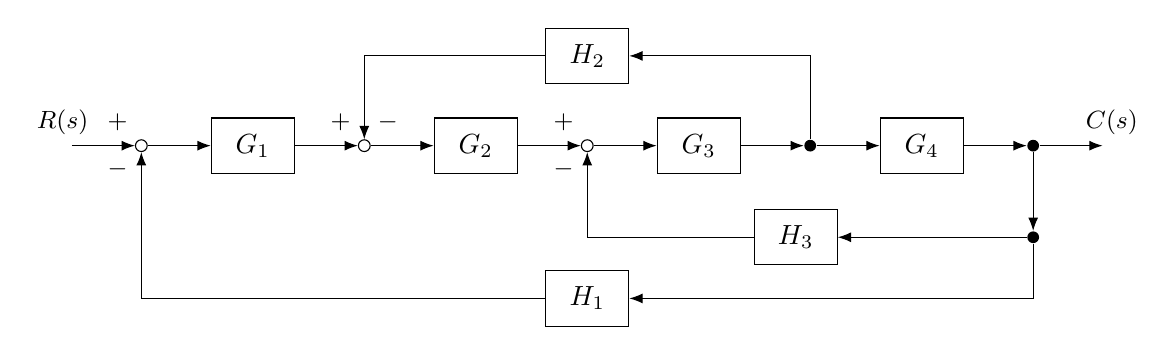
\begin{tikzpicture}[auto, node distance=0.8cm and 0.8cm, >=Latex]

      % --- 横並び:主系列ノード ---
      \node at (0,0) (input) {};
      \node[circle, draw, inner sep=1.5pt, right=of input] (sum1) {};         % 合流1
      \node[block, right=of sum1] (G1) {$G_1$};
      \node[circle, draw, inner sep=1.5pt, right=of G1] (sum2) {};            % 合流2
      \node[block, right=of sum2] (G2) {$G_2$};
      \node[circle, draw, inner sep=1.5pt, right=of G2] (sum3) {};            % 合流3
      \node[block, right=of sum3] (G3) {$G_3$};
      \node[circle, fill=black, inner sep=1.5pt, right=of G3] (branch1) {};   % 分岐1
      \node[block, right=of branch1] (G4) {$G_4$};
      \node[circle, fill=black, inner sep=1.5pt, right=of G4] (branch2) {};   % 分岐2
      \node[right=of branch2] (output) {};
  
      % --- 上・下ノード配置 ---
      \node[block, above=0.7cm of sum3] (H2) {$H_2$};                       % 合流3の上:H2
      \node[circle, fill=black, inner sep=1.5pt, below=1.0cm of branch2] (branch3) {}; % 分岐3
      \node[block, left=2.4cm of branch3] (H3) {$H_3$};                     % 分岐3の左
      \node[block, below=1.5cm of sum3] (H1) {$H_1$};                       % 合流3の下(H3より下)
  
      % === 主経路 ===
      \draw[->] (input) -- (sum1);
      \draw[->] (sum1) -- (G1);
      \draw[->] (G1) -- (sum2);
      \draw[->] (sum2) -- (G2);
      \draw[->] (G2) -- (sum3);
      \draw[->] (sum3) -- (G3);
      \draw[->] (G3) -- (branch1);
      \draw[->] (branch1) -- (G4);
      \draw[->] (G4) -- (branch2);
      \draw[->] (branch2) -- (output);
  
      % === 分岐ルート ===
      \draw[->] (branch1) |- (H2);              % 分岐1 → H2
      \draw[->] (H2) -| (sum2);                 % H2 → 合流2
  
      \draw[->] (branch2) -- (branch3);         % 分岐2 → 分岐3
      \draw[->] (branch3) -- (H3);              % 分岐3 → H3
      \draw[->] (H3) -| (sum3);                 % H3 → 合流3
  
      \draw[->] (branch3) |- (H1);              % 分岐3 → H1(下)
      \draw[->] (H1) -| (sum1);                 % H1 → 合流1
  
      % --- 加算記号配置 ---
      \node at ($(sum1)+(-0.3,0.3)$) {\small $+$};
      \node at ($(sum1)+(-0.3,-0.3)$) {\small $-$};
  
      \node at ($(sum2)+(-0.3,0.3)$) {\small $+$};
      \node at ($(sum2)+(+0.3,+0.3)$) {\small $-$};
  
      \node at ($(sum3)+(-0.3,0.3)$) {\small $+$};
      \node at ($(sum3)+(-0.3,-0.3)$) {\small $-$};
  
      % --- その他記号配置 ---
      \node at ($(sum1)+(-1.0,0.3)$) {\small $R(s)$};
      \node at ($(branch2)+(1.0,0.3)$) {\small $C(s)$};
  
  \end{tikzpicture}
  \end{center}
  \vspace{2mm}
  }]

  \begin{center}
    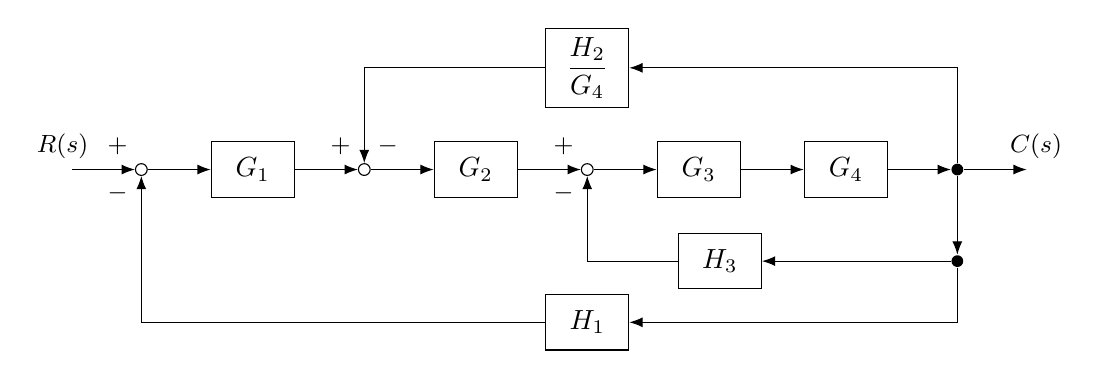
\begin{tikzpicture}[auto, node distance=0.8cm and 0.8cm, >=Latex]
    
      % --- 横並び:主系列ノード ---
      \node at (0,0) (input) {};
      \node[circle, draw, inner sep=1.5pt, right=of input] (sum1) {};         
      \node[block, right=of sum1] (G1) {$G_1$};
      \node[circle, draw, inner sep=1.5pt, right=of G1] (sum2) {};            
      \node[block, right=of sum2] (G2) {$G_2$};
      \node[circle, draw, inner sep=1.5pt, right=of G2] (sum3) {};            
      \node[block, right=of sum3] (G3) {$G_3$};
      \node[block, right=of G3] (G4) {$G_4$};
      \node[circle, fill=black, inner sep=1.5pt, right=of G4] (branch2) {};   % ← 分岐1と統合
      \node[right=of branch2] (output) {};
    
      % --- 上・下ノード配置 ---
      \node[block, above=0.7cm of sum3] (H2divG4) {$\dfrac{H_2}{G_4}$};    % ← H2/G4(上)
      \node[circle, fill=black, inner sep=1.5pt, below=1.0cm of branch2] (branch3) {};
      \node[block, left=2.4cm of branch3] (H3) {$H_3$};
      \node[block, below=1.5cm of sum3] (H1) {$H_1$};
    
      % === 主経路 ===
      \draw[->] (input) -- (sum1);
      \draw[->] (sum1) -- (G1);
      \draw[->] (G1) -- (sum2);
      \draw[->] (sum2) -- (G2);
      \draw[->] (G2) -- (sum3);
      \draw[->] (sum3) -- (G3);
      \draw[->] (G3) -- (G4);
      \draw[->] (G4) -- (branch2);
      \draw[->] (branch2) -- (output);
    
      % === 分岐ルート ===
      \draw[->] (branch2) |- (H2divG4);      % 上:H2 / G4
      \draw[->] (H2divG4) -| (sum2);
    
      \draw[->] (branch2) -- (branch3);
      \draw[->] (branch3) -- (H3);
      \draw[->] (H3) -| (sum3);
    
      \draw[->] (branch3) |- (H1);
      \draw[->] (H1) -| (sum1);
    
      % --- 加算記号配置 ---
      \node at ($(sum1)+(-0.3,0.3)$) {\small $+$};
      \node at ($(sum1)+(-0.3,-0.3)$) {\small $-$};
    
      \node at ($(sum2)+(-0.3,0.3)$) {\small $+$};
      \node at ($(sum2)+(+0.3,+0.3)$) {\small $-$};
    
      \node at ($(sum3)+(-0.3,0.3)$) {\small $+$};
      \node at ($(sum3)+(-0.3,-0.3)$) {\small $-$};
    
      % --- ラベル配置 ---
      \node at ($(sum1)+(-1.0,0.3)$) {\small $R(s)$};
      \node at ($(branch2)+(1.0,0.3)$) {\small $C(s)$};
    
    \end{tikzpicture}


    \vspace{2mm}
      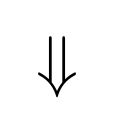
\begin{tikzpicture}
        \node {\Huge$\Downarrow$};
      \end{tikzpicture}
    \vspace{2mm}


    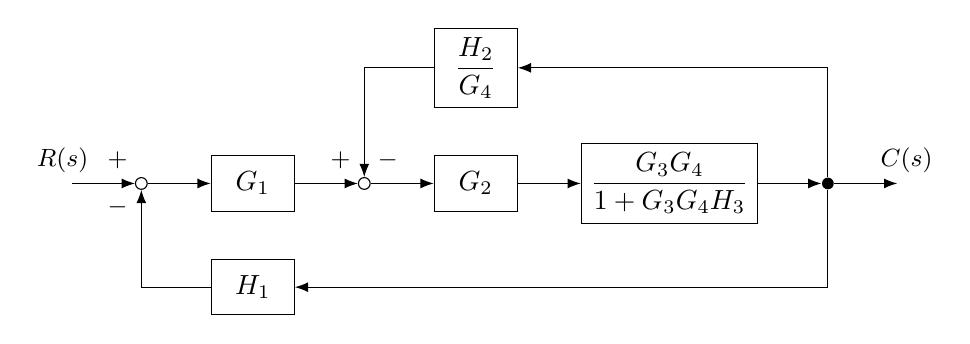
\begin{tikzpicture}[auto, node distance=0.8cm and 0.8cm, >=Latex]
    
      % --- 横並び:主系列ノード ---
      \node at (0,0) (input) {};
      \node[circle, draw, inner sep=1.5pt, right=of input] (sum1) {};         
      \node[block, right=of sum1] (G1) {$G_1$};
      \node[circle, draw, inner sep=1.5pt, right=of G1] (sum2) {};            
      \node[block, right=of sum2] (G2) {$G_2$};
      \node[block, right=of G2] (G34H3) {$\dfrac{G_3 G_4}{1 + G_3 G_4 H_3}$};  % 合成済ブロック
      \node[circle, fill=black, inner sep=1.5pt, right=of G34H3] (branch2) {};
      \node[right=of branch2] (output) {};
    
      % --- 上・下ノード配置 ---
      \node[block, above=0.6cm of G2] (H2divG4) {$\dfrac{H_2}{G_4}$};    % H₂/G₄(変更なし)
      \node[block, below=0.6cm of G1] (H1) {$H_1$};
    
      % === 主経路 ===
      \draw[->] (input) -- (sum1);
      \draw[->] (sum1) -- (G1);
      \draw[->] (G1) -- (sum2);
      \draw[->] (sum2) -- (G2);
      \draw[->] (G2) -- (G34H3);
      \draw[->] (G34H3) -- (branch2);
      \draw[->] (branch2) -- (output);
    
      % === 分岐ルート ===
      \draw[->] (branch2) |- (H2divG4);
      \draw[->] (H2divG4) -| (sum2);
    
      \draw[->] (branch2) |- (H1);
      \draw[->] (H1) -| (sum1);
    
      % --- 加算記号配置 ---
      \node at ($(sum1)+(-0.3,0.3)$) {\small $+$};
      \node at ($(sum1)+(-0.3,-0.3)$) {\small $-$};
    
      \node at ($(sum2)+(-0.3,0.3)$) {\small $+$};
      \node at ($(sum2)+(+0.3,+0.3)$) {\small $-$};
    
      % --- ラベル配置 ---
      \node at ($(sum1)+(-1.0,0.3)$) {\small $R(s)$};
      \node at ($(branch2)+(1.0,0.3)$) {\small $C(s)$};
    
    \end{tikzpicture}

    \vspace{2mm}
      \begin{tikzpicture}
        \node {\Huge$\Downarrow$};
      \end{tikzpicture}
    \vspace{2mm}


    \begin{tikzpicture}[auto, node distance=0.8cm and 0.8cm, >=Latex]
    
      % --- 横並び:主系列ノード ---
      \node at (0,0) (input) {};
      \node[circle, draw, inner sep=1.5pt, right=of input] (sum1) {};         
      \node[block, right=of sum1] (G1) {$G_1$};
      \node[block, right=of G1] (G234) {$\dfrac{G_2 G_3 G_4}{1 + G_3 G_4 H_3 + G_2 G_3 H_2}$}; % 合成済ブロック
      \node[circle, fill=black, inner sep=1.5pt, right=of G234] (branch2) {};
      \node[right=of branch2] (output) {};
    
      % --- 下ノード配置(H1のみ) ---
      \node[block, below=0.6cm of G1] (H1) {$H_1$};
    
      % === 主経路 ===
      \draw[->] (input) -- (sum1);
      \draw[->] (sum1) -- (G1);
      \draw[->] (G1) -- (G234);
      \draw[->] (G234) -- (branch2);
      \draw[->] (branch2) -- (output);
    
      % === フィードバック:H1のみ残す ===
      \draw[->] (branch2) |- (H1);
      \draw[->] (H1) -| (sum1);
    
      % --- 加算記号配置 ---
      \node at ($(sum1)+(-0.3,0.3)$) {\small $+$};
      \node at ($(sum1)+(-0.3,-0.3)$) {\small $-$};
    
      % --- ラベル配置 ---
      \node at ($(sum1)+(-1.0,0.3)$) {\small $R(s)$};
      \node at ($(branch2)+(1.0,0.3)$) {\small $C(s)$};
    
    \end{tikzpicture}

    \vspace{2mm}
      \begin{tikzpicture}
        \node {\Huge$\Downarrow$};
      \end{tikzpicture}
    \vspace{2mm}

    \begin{tikzpicture}[auto, node distance=1.5cm and 1.5cm, >=Latex]
    
      % --- ノード構成 ---
      \node at (0,0) (input) {};
      \node[block, right=of input] (Gfinal) {$\dfrac{G_1 G_2 G_3 G_4}{1 + G_3 G_4 H_3 + G_2 G_3 H_2 + G_1 G_2 G_3 G_4 H_1}$};
      \node[right=of Gfinal] (output) {};
    
      % --- 経路 ---
      \draw[->] (input) -- (Gfinal);
      \draw[->] (Gfinal) -- (output);
    
      % --- ラベル ---
      \node at ($(input)+(0,0.3)$) {\small $R(s)$};
      \node at ($(output)+(0,0.3)$) {\small $C(s)$};
    
    \end{tikzpicture}

    \end{center}
  




    
    

\end{tcolorbox}
% --------------- [50] --------------- 済
\begin{tcolorbox}[title={[50] ブロック線図を簡単にせよ. 
  \vspace{-2mm}
  \begin{center}
    \begin{tikzpicture}[auto, node distance=0.8cm and 0.8cm, >=Latex]

      % --- 横並びの主系列ノード ---
      \node at (0,0) (input) {};
      \node[circle, draw, inner sep=1.5pt, right=of input] (sum1) {};         % 合流1
      \node[block, right=of sum1] (G1) {$G_1$};
      \node[circle, draw, inner sep=1.5pt, right=of G1] (sum2) {};            % 合流2
      \node[block, right=of sum2] (G2) {$G_2$};
      \node[circle, fill=black, inner sep=1.5pt, right=of G2] (branch1) {};   % 分岐1
      \node[block, right=of branch1] (G3) {$G_3$};
      \node[circle, fill=black, inner sep=1.5pt, right=of G3] (branch2) {};   % 分岐2
      \node[right=of branch2] (output) {};
    
      % --- 合流3(sum1の下) ---
      \node[circle, draw, inner sep=1.5pt, below=0.7cm of sum1] (sum3) {};    % 合流3
    
      % === 経路 ===
      \draw[->] (input) -- (sum1);
      \draw[->] (sum1) -- (G1);
      \draw[->] (G1) -- (sum2);
      \draw[->] (sum2) -- (G2);
      \draw[->] (G2) -- (branch1);
      \draw[->] (branch1) -- (G3);
      \draw[->] (G3) -- (branch2);
      \draw[->] (branch2) -- (output);
    
      \draw[->] (branch1) |- (sum3);      % 分岐1 → 合流3
      \draw[->] (sum3) -- (sum1);         % 合流3 → 合流1
    
      \draw[->] (branch2) |- ++(0,-1.5) -| (sum3);   % 分岐2 → 合流3(下経路)
      \draw[->] (branch2) |- ++(0,0.8) -| (sum2);    % 分岐2 → 合流2(上経路)
    
      % --- 加算記号配置 ---
      \node at ($(sum1)+(-0.3,0.3)$) {\small $+$};
      \node at ($(sum1)+(-0.3,-0.3)$) {\small $-$};
      \node at ($(sum2)+(-0.3,0.3)$) {\small $+$};
      \node at ($(sum2)+(0.3,0.3)$) {\small $-$};
      \node at ($(sum3)+(0.3,0.3)$) {\small $+$};
      \node at ($(sum3)+(-0.3,-0.3)$) {\small $+$};
    
      % --- その他記号配置 ---
      \node at ($(sum1)+(-0.8,0.3)$) {\small $u$};
      \node at ($(branch2)+(0.8,0.3)$) {\small $y$};
    
  \end{tikzpicture}
  \end{center}
  \vspace{1mm}
  }]

  \begin{center}
    \begin{tikzpicture}[auto, node distance=0.8cm and 0.8cm, >=Latex]
    
      % --- 横並び:主系列ノード ---
      \node at (0,0) (input) {};
      \node[circle, draw, inner sep=1.5pt, right=of input] (sum1) {};         % 合流1
      \node[block, right=of sum1] (G1) {$G_1$};
      \node[circle, draw, inner sep=1.5pt, right=of G1] (sum2) {};            % 合流2
      \node[block, right=of sum2] (G2) {$G_2$};
      \node[block, right=of G2] (G3) {$G_3$};
      \node[circle, fill=black, inner sep=1.5pt, right=of G3] (branch1) {};   % 分岐1をG3の右に移動
      \node[circle, fill=black, inner sep=1.5pt, right=of branch1] (branch2) {}; 
      \node[right=of branch2] (output) {};
    
      % --- 合流3(sum1の下) ---
      \node[circle, draw, inner sep=1.5pt, below=1.15cm of sum1] (sum3) {};    % 合流3
    
      % --- G2の下に 1/G3 ノード追加 ---
      \node[block, below=0.3cm of G2] (invG3) {$\dfrac{1}{G_3}$};
    
      % === 主系列 ===
      \draw[->] (input) -- (sum1);
      \draw[->] (sum1) -- (G1);
      \draw[->] (G1) -- (sum2);
      \draw[->] (sum2) -- (G2);
      \draw[->] (G2) -- (G3);
      \draw[->] (G3) -- (branch1);
      \draw[->] (branch1) -- (branch2);
      \draw[->] (branch2) -- (output);
    
      % === 分岐ルート(新しい分岐1 → 1/G3 → 合流3)===
      \draw[->] (branch1) |- (invG3);
      \draw[->] (invG3) -- (sum3);
      \draw[->] (sum3) -- (sum1);
    
      % === 既存の分岐2からのフィードバックルート ===
      \draw[->] (branch2) |- ++(0,-2.2) -| (sum3);   % 分岐2 → 合流3(下経路)
      \draw[->] (branch2) |- ++(0,1.2) -| (sum2);    % 分岐2 → 合流2(上経路)
    
      % --- 加算記号配置 ---
      \node at ($(sum1)+(-0.3,0.3)$) {\small $+$};
      \node at ($(sum1)+(-0.3,-0.3)$) {\small $-$};
    
      \node at ($(sum2)+(-0.3,0.3)$) {\small $+$};
      \node at ($(sum2)+(0.3,0.3)$) {\small $-$};
    
      \node at ($(sum3)+(0.3,0.3)$) {\small $+$};
      \node at ($(sum3)+(-0.3,-0.3)$) {\small $+$};
    
      % --- ラベル配置 ---
      \node at ($(sum1)+(-0.8,0.3)$) {\small $u$};
      \node at ($(branch2)+(0.8,0.3)$) {\small $y$};
    
    \end{tikzpicture}


  \vspace{2mm}
    \begin{tikzpicture}
      \node {\Huge$\Downarrow$};
    \end{tikzpicture}
  \vspace{2mm}


    \begin{tikzpicture}[auto, node distance=0.8cm and 0.8cm, >=Latex]
    
      % --- 横並び:主系列ノード ---
      \node at (0,0) (input) {};
      \node[circle, draw, inner sep=1.5pt, right=of input] (sum1) {};         
      \node[block, right=of sum1] (G1) {$G_1$};
      \node[circle, draw, inner sep=1.5pt, right=of G1] (sum2) {};            
      \node[block, right=of sum2] (G2) {$G_2$};
      \node[block, right=of G2] (G3) {$G_3$};
      \node[circle, fill=black, inner sep=1.5pt, right=of G3] (branch2) {}; 
      \node[right=of branch2] (output) {};
    
      % --- 新しいフィードバックブロック(1 + 1/G3) ---
      \node[block, below=0.8cm of G2] (feedback) {$1 + \dfrac{1}{G_3}$};
    
      % === 主系列 ===
      \draw[->] (input) -- (sum1);
      \draw[->] (sum1) -- (G1);
      \draw[->] (G1) -- (sum2);
      \draw[->] (sum2) -- (G2);
      \draw[->] (G2) -- (G3);
      \draw[->] (G3) -- (branch2);
      \draw[->] (branch2) -- (output);
    
      % === 合成済みフィードバックルート ===
      \draw[->] (branch2) |- (feedback);
      \draw[->] (feedback) -| (sum1);
    
      % === 残るフィードバック(上) ===
      \draw[->] (branch2) |- ++(0,1.2) -| (sum2);
    
      % --- 加算記号配置 ---
      \node at ($(sum1)+(-0.3,0.3)$) {\small $+$};
      \node at ($(sum1)+(-0.3,-0.3)$) {\small $-$};
    
      \node at ($(sum2)+(-0.3,0.3)$) {\small $+$};
      \node at ($(sum2)+(0.3,0.3)$) {\small $-$};
    
      % --- ラベル配置 ---
      \node at ($(sum1)+(-0.8,0.3)$) {\small $u$};
      \node at ($(branch2)+(0.8,0.3)$) {\small $y$};
    
    \end{tikzpicture}


  \vspace{2mm}
    \begin{tikzpicture}
      \node {\Huge$\Downarrow$};
    \end{tikzpicture}
  \vspace{2mm}


    \begin{tikzpicture}[auto, node distance=0.8cm and 0.8cm, >=Latex]
      
        % --- 横並び:主系列ノード ---
        \node at (0,0) (input) {};
        \node[circle, draw, inner sep=1.5pt, right=of input] (sum1) {};
        \node[block, right=of sum1] (G1) {$G_1$};
        \node[block, right=of G1] (G23fb) {$\dfrac{G_2 G_3}{1 + G_2 G_3}$}; % 合成ブロック
        \node[circle, fill=black, inner sep=1.5pt, right=of G23fb] (branch2) {};
        \node[right=of branch2] (output) {};
      
        % --- フィードバックブロック(1 + 1/G₃) ---
        \node[block, below=0.8cm of G23fb] (feedback) {$1 + \dfrac{1}{G_3}$};
      
        % === 主系列 ===
        \draw[->] (input) -- (sum1);
        \draw[->] (sum1) -- (G1);
        \draw[->] (G1) -- (G23fb);
        \draw[->] (G23fb) -- (branch2);
        \draw[->] (branch2) -- (output);
      
        % === フィードバック(下) ===
        \draw[->] (branch2) |- (feedback);
        \draw[->] (feedback) -| (sum1);
      
        % --- 加算記号配置 ---
        \node at ($(sum1)+(-0.3,0.3)$) {\small $+$};
        \node at ($(sum1)+(-0.3,-0.3)$) {\small $-$};
      
        % --- ラベル配置 ---
        \node at ($(sum1)+(-0.8,0.3)$) {\small $u$};
        \node at ($(branch2)+(0.8,0.3)$) {\small $y$};
      
    \end{tikzpicture}

  \vspace{2mm}
    \begin{tikzpicture}
      \node {\Huge$\Downarrow$};
    \end{tikzpicture}
  \vspace{2mm}

    \begin{tikzpicture}[auto, node distance=1.5cm and 1.5cm, >=Latex]
    
      % --- ノード構成 ---
      \node at (0,0) (input) {};
      \node[block, right=of input] (Gfinal) {$\dfrac{G_1 G_2 G_3}{1 + G_2 G_3 + G_1 G_2 G_3 + G_1 G_2}$};
      \node[right=of Gfinal] (output) {};
    
      % --- 経路 ---
      \draw[->] (input) -- (Gfinal);
      \draw[->] (Gfinal) -- (output);
    
      % --- ラベル ---
      \node at ($(input)+(0.3,0.3)$) {\small $u$};
      \node at ($(output)+(-0.3,0.3)$) {\small $y$};
    
    \end{tikzpicture}

  \end{center}


    \vspace{-2mm}
最後の変形について
    \begin{align*}
      \frac{G_1 \cdot \dfrac{G_2 G_3}{1 + G_2 G_3}}{1 + G_1 \cdot \dfrac{G_2 G_3}{1 + G_2 G_3} \cdot \left(1 + \dfrac{1}{G_3} \right)}
      &= \frac{G_1 G_2 G_3}{1 + G_2 G_3 + G_1 G_2 G_3 \left(1 + \dfrac{1}{G_3} \right)} \\[1ex]
      &= \frac{G_1 G_2 G_3}{1 + G_2 G_3 + G_1 G_2 + G_1 G_2 G_3}
    \end{align*}

\end{tcolorbox}

\end{document}